% =====================================================================
%  main.tex — Ricostruzione LaTeX del volume (Michela Mollia)
%  Compilazione:  latexmk -pdf main.tex      (oppure: make)
%  Richiede biber per la bibliografia.
% =====================================================================
\documentclass[11pt,twoside,openany]{book}
\usepackage{stile}

\addbibresource{bibliografia.bib}

% --- Dati del frontespizio (dalla scansione di copertina e frontespizio) ---
\newcommand{\Autore}{Walter Branchi}
\newcommand{\Titolo}{I numeri della musica}
\newcommand{\SottotitoloA}{Elementi di calcolo degli intervalli}
\newcommand{\SottotitoloB}{e sistemi d'intonazione}
\newcommand{\Introduttore}{Michela Mollia}
\newcommand{\Editore}{edipan}

\begin{document}

% =====================================================================
%  FRONTESPIZIO (ricostruito — dati da confermare)
% =====================================================================
\frontmatter
\thispagestyle{empty}
\begin{center}
  \vspace*{1.2cm}
  {\Large \Autore\par}
  \vspace{2.4cm}
  {\fontsize{30}{34}\selectfont \Titolo\par}
  \vspace{0.45cm}
  {\LARGE \SottotitoloA\par}
  \vspace{0.18cm}
  {\LARGE \SottotitoloB\par}
  \vspace{2.6cm}
  {\large\bfseries Introduzione di \Introduttore\par}
  \vfill
  {\large\itshape \Editore\par}
  \vspace{1.2cm}
\end{center}
\clearpage

% =====================================================================
%  INDICE — spostato all'INIZIO (nell'originale era in fondo)
% =====================================================================
\tableofcontents
\cleardoublepage

% =====================================================================
%  CORPO
% =====================================================================
\mainmatter

% =====================================================================
%  Introduzione  (di Michela Mollia) — scansione p-01 .. p-04
%  Testo trascritto integralmente dalle immagini (de-ombreggiate).
% =====================================================================
\chapter*{Introduzione}
\addcontentsline{toc}{chapter}{Introduzione}
\markboth{Introduzione}{Introduzione}

Un sistema musicale è un'organizzazione di relazioni (intervalli) tra altezze
e inevitabilmente tali relazioni vengono rappresentate da numeri. Il calcolo
degli intervalli non è certo materia nuova, ma nemmeno estranea ad un certo
tipo di pensiero compositivo contemporaneo, come vedremo più avanti.

In effetti esso affonda le sue radici nell'antichità più remota. Pitagora da
Samo nel IV secolo a.C. ne aveva stabilito alcune delle regole fondamentali,
ma certamente civiltà musicali diverse, come ad esempio quella cinese, ne
conoscevano i principi: una corda viene suddivisa in parti via via sempre più
piccole, prima la metà, poi un terzo, un quarto\dots\ la scoperta di altezze
diverse le cui relazioni con la nota fondamentale sono le stesse con cui gli
armonici si mettono in rapporto l'uno con l'altro rispetto al fondamentale: ma
con una piccola grande differenza, inversamente proporzionali. Questa legge
semplice non è altro che il principio degli armonici riscontrato e formulato
solamente nel XVII secolo. È comunque sorprendente notarne l'antica intuizione.

L'estrema semplicità di questo generatore, che ancora non sa di musica, di
fantasia, di amore o di guerra, è però perfetta nella sua regolare disposizione
di leggi. Vale la pena ricordare come tale equilibrio venne poi ricercato nel
movimento degli astri, nelle forme geometriche più semplici, nel modo come la
natura ordina e costituisce i suoi organismi, dai più elementari ai più
complessi. A questo punto sarebbe fin troppo facile cantare non originali lodi
sulla meravigliosa unitarietà dell'universo. La nostra dimensione ha perduto,
purtroppo o no, questo legame, la consapevolezza di far parte di un unico tutto.
Abbiamo altre cose per le mani.

I nostri strumenti musicali sono molto più complicati, ma se togliamo loro le
accurate e sofisticate sovrastrutture di legno o metallo, troveremo la familiare
corda vibrante o l'inafferabilità della colonna d'aria. Questi oggetti sono per
lo più legati indissolubilmente a leggi e modelli fisico-musicali che hanno
provocato e permesso sia la loro realizzazione sia opere che di questi strumenti
facessero uso.

Quando anni fa il compositore cominciò a modellarsi la materia sonora
nell'ambito delle esperienze della musica concreta, era in un certo senso
ancora indifferente alla sua quantizzazione interna, lavorando più su aggregati
timbrici, più o meno evocativi, che su grandezze sonore su cui fosse oggetto una
rete di relazioni, se pure arbitraria, che costituisse un sistema. La dimensione
sonoro-compositiva muta, direi radicalmente, nel momento in cui si lavora con
generatori elettronici analogici e ancora di più, recentemente, con elaboratori
digitali che, tramite adeguati sistemi di conversione numerico/analogica, sono
in grado di sintetizzare qualsiasi forma d'onda.

Se a questo aggiungiamo la possibilità di creare di volta in volta dei sistemi
di intervalli che soddisfino le necessità espressive e compositive del momento
(aprendo magari la strada ad una grammatica degli intervalli) si può intravedere
un universo sonoro molto più sfaccettato e versatile di quanto il temperamento
equabile non abbia permesso.

In effetti, se a questo punto facciamo un'analisi musicologica dei sistemi di
intonazione che si sono imposti nella pratica musicale occidentale, vediamo che
soprattutto tre hanno avuto una rilevanza storica. Fino al XVI secolo ci si
avvale del sistema pitagorico, che considera solamente i numeri 1, 2, 3 e 4
(fondamentale, ottava, quinta e doppia ottava). Questa serie di numeri naturali
viene chiamata appunto \emph{Tetractys} pitagorica. Essa costituiva il nucleo
dal quale si faceva risalire la generazione e il susseguente ordinamento
armonico del mondo. I pitagorici concepivano il mondo come musicalmente
costituito e fissavano questo concetto con il termine \enquote{cosmo}.

Con il formarsi dell'armonia moderna questo sistema si rivelò essere di
difficile impiego, in quanto non facilitava un'organizzazione basata su accordi
(la consonanza perfetta non poteva essere di soli due suoni). Al contrario,
favoriva un contrappunto di linee indipendenti. Ed ecco perché la polifonia
primitiva, come pure quella del Medio Evo, è una polifonia di contrappunto,
guidata dal procedere melodico delle parti e non dai rapporti contenuti negli
accordi.

Altra caratteristica del sistema pitagorico è quella di avere il semitono
considerevolmente più piccolo di quello temperato, mentre tutti gli altri
intervalli risultano allargati. Questo provoca una tendenza molto forte di
alcuni di questi a risolvere su altri più semplici. Il sistema pitagorico è
quindi essenzialmente dinamico, accentua le differenze tra gli intervalli e
aumenta le dissonanze, che devono perentoriamente risolvere.

Il sistema cosiddetto zarliniano opera un allargamento armonico da 2, 3 suoni,
giungendo così al fattore 5 (terza maggiore). Questo intervallo rende l'accordo
più stabile, passando dal rapporto $81/64$ a quello più consonante di $5/4$.
L'armonia del XVI secolo liquida progressivamente il contrappunto e, smussando
le attrazioni intervallari pitagoriche, forma un tappeto di accordi consonanti
che fanno risaltare la melodia. Possiamo perciò dire che il sistema zarliniano
è, in tal senso, un sistema statico: la gerarchia dei cicli delle quinte finisce
per scomparire, la struttura cessa di essere do-fa-sol-do per diventare il
do-mi-sol-do.

Differentemente dai precedenti, il temperamento equabile non è né statico né
dinamico. Esso opera dei continui compromessi tra i due sistemi: un sistema
neutro nel quale, operando mentalmente continue correzioni degli intervalli, ci
muoviamo melodicamente verso il pitagorismo mentre per l'armonia ci rivolgiamo
al sistema zarliniano. Esso non impone nulla e permette tutto. D'altra parte
questa ambiguità ha permesso di suonare in tutte le tonalità, di modulare
rapidamente e fare uso dell'enarmonia in senso moderno. A quanto detto, se pur
brevemente, si può aggiungere di conseguenza come il passaggio nella storia
della musica da un sistema di intonazione ad un altro non sia un fatto
accidentale, ma uno degli elementi essenziali, la matrice determinante
dell'evoluzione del linguaggio musicale.

D'altra parte un compositore attento, come era senza dubbio Arnold Schoenberg,
nel suo saggio \emph{Problems of Harmony} del 1934 osservava come noi stiamo
provando ad esprimere armonie del 7, 9 e 11 in un sistema e con strumenti di
notazione formati soltanto per quelle del 3 e del 5, sottolineando sia
l'incapacità del temperamento equabile di reggere la spinta evolutiva di un
linguaggio musicale che stava cambiando, sia la contraddizione tra un operare,
diciamo così, avanzato, che però si serviva di un sistema nato per tutt'altre
esigenze.

A questo punto il saper trattare ed esporre, essenzialmente e non con la pretesa
di teorici, lo studio e la pratica riguardante il calcolo degli intervalli ci
sembra molto proficuo e in definitiva affascinante. Perlomeno per quella libertà
di definizione che oggi ci è permessa da mezzi come gli elaboratori, che
garantiscono la precisa realizzazione di qualsiasi grandezza voluta. Conoscendo
le caratteristiche dei vari sistemi di intonazione sceglieremo quelli, o parte
di quelli, più adatti alle nostre esigenze compositive.

Inoltre, dato che nel campo della musica elettronica non esistono suoni
preformati, è ancora più evidente come chi opera in questo ambito debba, per
forza di cose, predisporsi tutti i livelli della composizione. E dato che ai
calcolatori si parla con i numeri (almeno nella maggior parte dei casi) si può
ritrovare come estensione quella antica concezione di numero e suono in cui uno
è espressione dell'altro e dove qualità e quantità si trovano per l'unica volta
unite. In altre parole, quando parliamo di \enquote{ottava} ci riferiamo
inequivocabilmente a quel certo intervallo, a quella precisa qualità
intervallare, ma, nello stesso tempo, a quella precisa quantità, misurazione se
vogliamo, di corda o colonna d'aria.

Chiediamo ad un musicista di misurare una corda e di indicare la sua esatta metà
senza l'uso di un sistema di misurazione: questo calcolo verrà effettuato nella
maniera più empirica ed efficace, andandosi a cercare cioè l'ottava. Si potrebbe
dire perciò con Curt Sachs: \enquote{Il suono non ha relazione diretta con altre
forme di percezione, avendo rispondenza solo con gli aspetti più astratti della
realtà: il numero e la misura}.

Il calcolo degli intervalli rappresenta in musica ciò che il problema della
quadratura del cerchio è in geometria: un calcolo che si avvicina sempre più al
segno di infinito. D'altra parte, se è vero che la serie dei numeri è
praticamente illimitata, possiamo pensare ad una illimitata serie di intervalli?
Si può dire che il nostro orecchio pone delle condizioni di discriminabilità: la
minima differenza di \cents{6} costituisce una soglia più o meno generalizzabile
per il riconoscimento degli intervalli. Certamente, comunque, con un computer
potremmo conoscere e cogliere quelle minime differenze, giungendo, perché no, ad
un tipo diverso di espressività, che sembrava estranea ad uno strumento da molti
considerato una macchina.

Scopo quindi di questa trattazione è quello di fornire gli elementi e principi
essenziali di calcolo degli intervalli. Questa conoscenza può essere di grande
importanza sia per un'analisi più appropriata dei sistemi di intonazione già
messi in pratica, che come punto di partenza per la creazione di nuovi.

Attraverso queste pagine è possibile seguire il cammino della musica così come
\enquote{suonava} tanto tempo fa, che è sicuramente molto diverso da quello di
oggi. Il concetto di intervallo, quindi, non è da leggersi come irrevocabilmente
legato alle \enquote{note}, bensì va inteso nel senso più allargato di
proporzione, distanza, emozione.

\firma{Michela Mollia}

% =====================================================================
%  Capitolo 1 — Elementi di calcolo degli intervalli
%  Apertura (p-05, p-06) trascritta integralmente.
%  Sezioni 1.1-1.3.3 (da p-07 in poi): DA TRASCRIVERE.
% =====================================================================
\chapter{Elementi di calcolo degli intervalli}

Esistono diversi modi attraverso i quali si può procedere all'investigazione
sulla natura e calcolo degli intervalli e tra questi, da quasi 3000 anni,
l'impiego del monocordo si è rivelato particolarmente efficace per esperimenti
e dimostrazioni di carattere scientifico e musicale. Il monocordo, come dice il
nome stesso, è uno strumento formato da una corda tesa tra due ponticelli su
una cassa di risonanza e da un ulteriore ponticello mobile che viene utilizzato
per dividere la corda in porzioni diverse a seconda dell'intervallo desiderato.

L'altezza di un suono generato su un monocordo dipende dal peso per unità di
lunghezza della corda (materiale e diametro), tensione e lunghezza. Queste
grandezze sono alla base delle quattro leggi fondamentali riguardanti la corda
vibrante in relazione all'altezza del suono emesso:

\begin{elenco}
  \item il numero di periodi per secondo è inversamente proporzionale alla
        lunghezza della corda;
  \item il numero di periodi per secondo è proporzionale alla radice quadrata
        della tensione alla quale la corda è soggetta;
  \item il numero di periodi per secondo varia inversamente allo spessore della
        corda;
  \item il numero di periodi per secondo è inversamente proporzionale alla
        radice quadrata della densità della corda.
\end{elenco}


Per il nostro scopo terremo conto soltanto della lunghezza della corda,
ritenendo costanti gli altri parametri. Ora, considerando la prima legge sulla
corda vibrante, avremo che se la corda è lunga un metro e oscilla con una
frequenza di 500 periodi al secondo, la stessa corda con il ponticello mobile
disposto alla sua metà ($1/2$) darà una frequenza pari a
$500 \times \frac{2}{1} = 1000$ periodi al secondo e, ancora, ridotta a $2/3$
della lunghezza totale, darà $500 \times \frac{3}{2} = 750$ periodi al secondo,
e così via. Nel calcolo della frequenza di un intervallo i termini del rapporto
che la definiscono verranno posti in modo tale da avere il valore più grande al
numeratore, mentre per determinare la lunghezza della corda vibrante il valore
più grande si troverà al denominatore. Poniamo di avere una corda lunga un metro
con una frequenza propria di 500~Hz: per sapere sia la frequenza relativa che il
punto della corda dove si dovrà disporre il ponticello mobile per trovare la sua
quinta ($3/2$) avremo:
\[
  500~\text{Hz} \times \tfrac{3}{2} = 750~\text{Hz}
  \qquad
  1~\text{m} \times \tfrac{2}{3} = 66{,}6~\text{cm}
\]

Un \emph{intervallo} tra due frequenze viene definito dal rapporto, o dal
quoziente, tra le due frequenze che lo formano. Per esempio, l'intervallo o la
distanza tra una frequenza di 500~Hz e una di 800~Hz è espresso dal rapporto
$8/5$ oppure dal suo quoziente $1{,}6$.

Nel calcolo teorico degli intervalli le altezze reali sono immaginarie: una nota
arbitraria, normalmente DO, viene scelta come punto di partenza e ad essa è
assegnato un valore di frequenza $1$. In pratica il calcolo degli intervalli
viene effettuato considerando essenzialmente tre intervalli elementari:
\[
  \text{ottava} = O \qquad
  \text{quinta} = Q \qquad
  \text{terza maggiore} = T
\]

Esperimenti iniziati da Pitagora da Samo già nel VI secolo a.C. fornirono le
seguenti regole:

\begin{elenco}
  \item la frequenza di un suono è $n$, quella dell'ottava è $2n$, della quinta
        $\frac{3}{2}n$ e della terza maggiore $\frac{5}{4}n$ (è da notare che
        questi intervalli sono i primi tre componenti con una propria identità
        della serie degli armonici: $2/1$ ottava, $3/1$ dodicesima-quinta,
        $5/1$ diciassettesima-terza maggiore);
  \item gli intervalli si \emph{addizionano} moltiplicando le loro rispettive
        frazioni. Quindi, per esempio, l'intervallo di dodicesima (quinta
        all'ottava superiore) è uguale a
        $Q + O = \frac{3}{2} \times \frac{2}{1} = \frac{3}{1}$;
        l'intervallo di settima maggiore è uguale a
        $Q + T = \frac{3}{2} \times \frac{5}{4} = \frac{15}{8}$;
  \item un intervallo si \emph{sottrae} moltiplicando la rispettiva frazione
        invertita. Per esempio, l'intervallo di quarta è uguale a
        $O - Q = \frac{2}{1} \times \frac{2}{3} = \frac{4}{3}$ e l'intervallo di
        terza minore è uguale a
        $Q - T = \frac{3}{2} \times \frac{4}{5} = \frac{6}{5}$.
\end{elenco}

Nel calcolo degli intervalli complessi si può procedere ad una semplificazione
che consiste nel non considerare l'intervallo nell'ambito del rapporto $2/1$,
trascurando cioè il fattore 2. Così facendo la quinta diviene semplicemente $3$
e la terza maggiore $5$. Naturalmente, con questo procedimento, le ottave
risultanti non sono corrette nel senso della posizione dell'intervallo
nell'ambito di una stessa ottava. Comunque questa piccola difficoltà può essere
facilmente risolta moltiplicando il risultato ottenuto per una potenza di 2
($2, 4, 8, \tfrac{1}{2}, \tfrac{1}{4}, \tfrac{1}{8}$ ecc.).

Grazie a questo calcolo si può far rientrare l'intervallo nell'ottava. Ad
esempio nel calcolo della settima maggiore si avrà:
\[
  Q + T = 3 \times 5 = 15 \times \tfrac{1}{8} = \tfrac{15}{8}
\]

Un intervallo è contenuto nell'ottava quando il valore del denominatore della
sua frazione è superiore alla metà del valore del numeratore e quindi il
risultato del quoziente è compreso tra 1 e 2.

Questo sistema di calcolo degli intervalli è particolarmente conveniente quando
si deve stabilire l'intervallo rispetto ad un rapporto dato. Per esempio, quale
intervallo è rappresentato da $9/8$? Trascurando tutte le potenze di 2 (quindi
8) troviamo che esso è formato da $3 \times 3 = 9$ cioè $Q + Q = $~RE, quindi
l'intervallo è di un tono. Oppure determinare l'intervallo corrispondente al
rapporto $25/18$:
\[
  \frac{25}{18} = \frac{5 \times 5}{3 \times 3 \times 2} = 2T - 2Q = \text{FA}\sharp
\]
e ancora, trovare l'intervallo corrispettivo al rapporto $45/32$:
\[
  45 = 3 \times 3 \times 5 = 2Q + T = \text{FA}\sharp
\]

Questo FA$\sharp$ non può essere uguale al primo e la ragione di tale
differenza, un \emph{comma sintonico}, è da ricercarsi nel fatto che il calcolo
di uno stesso intervallo può essere eseguito con diverse combinazioni di ottave,
quinte e terze maggiori.\footnote{I termini ottava, quinta e terza sono relativi
ai gradi della scala eptatonica dove, per esempio, il rapporto $2/1$ (ottava)
corrisponde appunto al suo ottavo grado. Chiaramente, per altre scale, come la
pentatonica o la dodecatonica, essi sono totalmente impropri. I Greci chiamavano
l'intervallo tra la corda intera e la sua metà \emph{diapason}, termine che
tradotto letteralmente significa \emph{attraverso tutto}, \emph{attraverso
l'intero}, ossia attraverso l'intero spazio tonale le cui relazioni interne si
ripetono sempre uguali.} Il sistema più semplice per calcolare la differenza o
\emph{comma sintonico} tra i due FA$\sharp$ consiste nel sottrarre i due membri
che li rappresentano:
\[
  (2Q+T) - (2T-2Q) = 2Q + T - 2T + 2Q = 4Q - T =
\]
\[
  = \tfrac{3}{2} \times \tfrac{3}{2} \times \tfrac{3}{2} \times \tfrac{3}{2}
    \times \tfrac{4}{5} = \tfrac{81}{20} \times \tfrac{1}{4}
    = \frac{81}{80}\footnote{La scrittura per esteso è stata adottata per
    maggiore chiarezza, ma naturalmente l'espressione può essere indicata come:
    $\left(\frac{3}{2}\right)^{4} \times \frac{4}{5} =
     \frac{81}{20} \times \frac{1}{4} = \frac{81}{80}$.}
\]

$81/80$ è il rapporto che rappresenta il \emph{comma sintonico}.

Ecco il calcolo del \emph{comma sintonico} tra il tono grande $9/8$, comune sia
al sistema pitagorico che a quello naturale, e il tono piccolo $10/9$ presente
solo in quello naturale:
\[
  \text{tono grande} = \frac{9}{8} = 2Q = \frac{3}{2} \times \frac{3}{2}
    = \frac{9}{4} \times \frac{1}{2} = \frac{9}{8}
\]
\[
  \text{tono piccolo} = \frac{10}{9} = O + T - 2Q = \frac{2}{1} \times
    \frac{5}{4} \times \frac{4}{9} = \frac{40}{36} = \frac{10}{9}
\]
\[
  \text{quindi} \quad (2Q) - (O - T - 2Q) = 2Q - O + T + 2Q = 4Q - O - T =
\]
\[
  = \tfrac{3}{2} \times \tfrac{3}{2} \times \tfrac{3}{2} \times \tfrac{3}{2}
    \times \tfrac{1}{2} \times \tfrac{4}{5} = \frac{324}{160} = \frac{81}{80}
\]
% [sic] Nell'originale il risultato intermedio 324/160 è ridotto a 81/80
% (la riduzione corretta sarebbe 81/40): refuso riprodotto fedelmente.

Il \emph{Comma} e lo \emph{Schisma} sono quei valori di scarto in altezza che si
vengono a determinare nel calcolo degli intervalli\footnote{Tale calcolo rimane
inalterato indipendentemente dalla natura del generatore, sia esso corda
vibrante o colonna d'aria in un tubo.} quando una stessa altezza, come abbiamo
già avuto modo di vedere, viene ottenuta attraverso la differente combinazione
di ottave, quinte e terze maggiori.\footnote{Tutti gli intervalli, ad eccezione
dell'ottava che è comune a tutti i sistemi di intonazione, sono da considerarsi
come riferiti al sistema naturale e non a quello del temperamento equabile.}

Il \emph{Comma ditonico} o \emph{pitagorico} si verifica nella differenza tra 12
quinte e 7 ottave $(12Q - 7O)$:
\[
  \left(\frac{3}{2}\right)^{12} \times \left(\frac{1}{2}\right)^{7}
  = \frac{3^{12}}{2^{19}} = \frac{531441}{524288}
  = 23{,}5~\text{cents}\footnote{Per il calcolo dei cents vedi
  \emph{Intervalli logaritmici}.}
\]

Il \emph{Comma sintonico} o \emph{Didimico} si verifica nella differenza tra 4
quinte e la somma di 2 ottave più una terza maggiore $(4Q - 2O - 1T)$:
\[
  \left(\frac{3}{2}\right)^{4} \times \frac{4}{5} \times
  \left(\frac{1}{2}\right)^{2} = \frac{3^{4}}{2^{4} \times 5}
  = \frac{81}{80} = 21{,}5~\text{cents}
\]

Lo \emph{Schisma} si verifica nella differenza tra 8 quinte più una terza
maggiore e 5 ottave $(8Q + 1T - 5O)$:
\[
  \left(\frac{3}{2}\right)^{8} \times \frac{5}{4} \times
  \left(\frac{1}{2}\right)^{5} = \frac{3^{8} \times 5}{2^{15}}
  = \frac{32805}{32768} = 2~\text{cents}
\]

Il \emph{Diaschisma} si verifica nella differenza tra 3 ottave e la somma di 4
quinte più 2 terze maggiori $(3O - 4Q - 2T)$:
\[
  \left(\frac{2}{1}\right)^{3} \times \left(\frac{2}{3}\right)^{4} \times
  \left(\frac{4}{5}\right)^{2} = \frac{2^{11}}{3^{4} \times 5^{2}}
  = \frac{2048}{2025} = 19{,}5~\text{cents}
\]

Il \emph{comma ditonico} è anche la differenza tra i due semitoni della scala
diatonica pitagorica e il \emph{comma sintonico}, come visto precedentemente,
tra i due toni interi della scala naturale.

Lo \emph{schisma} è la differenza tra il \emph{comma ditonico} e quello
\emph{sintonico}, nonché tra il \emph{comma sintonico} e il \emph{diaschisma}:
\[
  \frac{3^{12}}{2^{19}} \times \frac{5 \times 2^{4}}{3^{4}}
  = \frac{3^{8} \times 5}{2^{15}}
\]
\[
  \frac{3^{4}}{2^{4} \times 5} \times \frac{3^{4} \times 5^{2}}{2^{11}}
  = \frac{3^{8} \times 5}{2^{15}}
\]

% =====================================================================
\section{Intervalli complementari}

Due intervalli si dicono complementari quando, moltiplicando le rispettive
frazioni, il risultato che si ottiene è $2/1$. Ad esempio, moltiplicando
$3/2 \times 4/3$ si otterrà:
\[
  \frac{3}{2} \times \frac{4}{3} = \frac{4}{2} = \frac{2}{1}
\]

Dato un intervallo, il complementare si ricava semplicemente invertendo i suoi
due termini, facendo però attenzione che la nuova frazione sia stata prima
semplificata (ridotta ai minimi termini) e che essa sia contenuta nell'ambito
dell'ottava. Ne risulta che il complementare di $81/80$ sarà $80/81$ che
riportato nell'ottava darà $160/81$. Pertanto:
\[
  \frac{81}{80} \times \frac{160}{81} = \frac{160}{80} = \frac{2}{1}
\]

Trovare il complementare di $800/729$: invertendo i termini della frazione
avremo $729/800$. Riportandola nell'ottava avremo $1458/800$ che, ridotta ai
minimi termini, risulterà $729/400$, quindi:
\[
  \frac{800}{729} \times \frac{729}{400} = \frac{800}{400} = \frac{2}{1}
\]

Naturalmente, l'intervallo complementare si può ottenere anche moltiplicando la
frazione che lo esprime per $1/2$ e invertendo poi il risultato ottenuto:
\[
  \frac{15}{8} \times \frac{1}{2} = \frac{15}{16} \quad\text{da cui}\quad
  \frac{16}{15}
\]

% =====================================================================
\section{Intervalli logaritmici}

L'impiego dei logaritmi può semplificare molto il calcolo degli intervalli.
Secondo l'equazione fondamentale dei logaritmi:
\[
  \log(A \times B) = \log A + \log B
\]
ne consegue che il logaritmo di un prodotto è uguale alla somma dei logaritmi
dei fattori. Vale a dire $\log 15 = \log 3 + \log 5$. Se perciò due intervalli
$i_1$ e $i_2$ sono rappresentati non dai loro rapporti di frequenza $f_1$ e
$f_2$ ma dai logaritmi dei simboli $\log f_1$ e $\log f_2$, il calcolo degli
intervalli viene effettuato con:
\[
  \log(f_1 \times f_2) = \log f_1 + \log f_2
\]

Si ottiene così che, se vengono usati gli intervalli logaritmici, l'addizione e
la sottrazione degli intervalli viene fatta in realtà addizionando e sottraendo
i simboli anziché moltiplicandoli o dividendoli. Il vantaggio principale
nell'impiego delle frequenze logaritmiche consiste nel fatto che uguali
intervalli musicali sono rappresentati da uguali distanze su una scala
geometrica.

\begin{figure}[htbp]
  \centering
  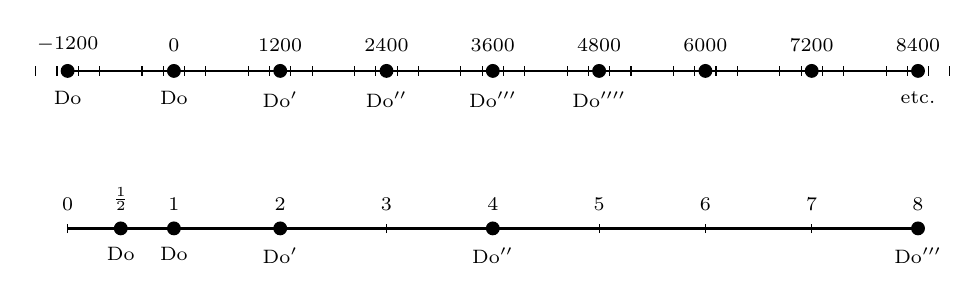
\begin{tikzpicture}[x=1.35cm,y=1cm]
    % --- (a) scala logaritmica (cents): le ottave sono equidistanti ---
    \draw[thick] (0,2) -- (8,2);
    \foreach \i in {0,...,8}{
      \foreach \k in {1,...,4}{\draw (\i-0.5+\k*0.2,1.94) -- (\i-0.5+\k*0.2,2.06);}
    }
    \foreach \i/\n/\d in {%
        0/$-1200$/Do, 1/$0$/Do, 2/$1200$/Do$'$, 3/$2400$/Do$''$,
        4/$3600$/Do$'''$, 5/$4800$/Do$''''$, 6/$6000$/{}, 7/$7200$/{},
        8/$8400$/etc.}{
      \filldraw (\i,2) circle (2.3pt);
      \node[above,font=\scriptsize] at (\i,2.12) {\n};
      \node[below,font=\scriptsize] at (\i,1.86) {\d};
    }
    % --- (b) scala lineare (frequenza): le ottave si allontanano ---
    \draw[thick] (0,0) -- (8,0);
    \foreach \i in {0,...,8}{\draw (\i,-0.06) -- (\i,0.06);}
    \draw (0.5,-0.06) -- (0.5,0.06);
    \foreach \x/\n in {0/$0$,0.5/$\frac12$,1/$1$,2/$2$,3/$3$,4/$4$,5/$5$,6/$6$,7/$7$,8/$8$}
      {\node[above,font=\scriptsize] at (\x,0.10) {\n};}
    \foreach \x/\d in {0.5/Do,1/Do,2/Do$'$,4/Do$''$,8/Do$'''$}{
      \filldraw (\x,0) circle (2.3pt);
      \node[below,font=\scriptsize] at (\x,-0.12) {\d};
    }
  \end{tikzpicture}
\end{figure}

Dall'esempio si vede come nella usuale scala logaritmica dei cents le varie
ottave sono indicate da cifre equidistanti, come $0$, $1200$, $2400$, $3600$
cents, mentre al contrario, nella scala lineare delle frequenze, le ottave sono
indicate dalle cifre $1$, $2$, $4$, $8$ ecc. Le frequenze logaritmiche sono
particolarmente importanti, se non indispensabili, in tutti i calcoli inerenti
intervalli temperati o microintervalli. Ad esempio, il temperamento equabile
consiste nella divisione dell'ottava in 12 intervalli (semitoni) equidistanti.
Poiché l'ottava ha la frequenza 2, abbiamo l'equazione
$\sqrt[12]{2}$,\footnote{Il calcolo della radice $n$-esima di un numero
$\sqrt[n]{a}$ si effettua con $a^{1/n}$. Per esempio, nel caso di
$\sqrt[12]{2}$ si procederà nel dividere 1 per l'indice del radicale:
$1/12 = 0{,}083333\ldots$, quindi si eleverà il radicando 2 per il risultato
ottenuto: $2^{0{,}083333\ldots} = 1{,}059463094$.} quindi $1{,}0594630943$. La
successiva potenza di questa cifra darà la frequenza dell'intervallo seguente
della scala temperata: $\text{RE} = 1{,}05946^{2} = 1{,}12246$,
$\text{RE}\sharp = 1{,}05946^{3} = 1{,}18919$ ecc.

Usando invece i logaritmi, gli intervalli della scala temperata possono essere
calcolati facilmente essendo essi tutti multipli del $\log$ dell'intervallo più
piccolo: $\log 1{,}0594630943 = 0{,}025085833$, quindi $\text{DO} = 0$,
$\text{DO}\sharp = 0{,}025085833$, $\text{RE} = 0{,}050171666$,
$\text{RE}\sharp = 0{,}075257499$ e così via fino all'ottava
$\text{DO'} = 0{,}301029957$.

L'unico inconveniente in questo sistema di calcolo è rappresentato dal fatto di
dover impiegare numeri così ingombranti. Tuttavia questa difficoltà può essere
facilmente evitata moltiplicando la scala per un determinato fattore. In questo
modo allargato si ottengono varie scale logaritmiche. La più diffusa è quella
studiata da Ellis [Alexander J. Ellis, 1814--1890] nella quale il fattore
allargato è dato da $1200/\!\log 2 = 3986{,}313714$, cosicché l'ottava viene
divisa esattamente in 1200 parti. L'unità, in questo sistema di misurazione, è
il \emph{cent}. Quindi, se l'ottava divisa in 12 semitoni equidistanti è uguale
a $1200$ cents, ogni semitono temperato avrà il valore di $100$ cents.

Un altro sistema logaritmico piuttosto comune è quello di Savart [Felix Savart,
1791--1841]. Anche con questa scala è possibile calcolare gli intervalli
logaritmici contenuti nell'ambito del rapporto $2/1$, ossia tra $0$ e $0{,}3010$.
In questo metodo il fattore allargato è uguale a $1000$, quindi tutte le cifre
vengono moltiplicate per $1000$ ottenendo così che l'ottava, anziché essere
$0{,}3010$, è uguale a $301$ savarts. Entrambi i sistemi sono molto efficaci per
calcolare qualsiasi tipo di intervallo musicale. Difatti, se consideriamo che il
semitono temperato nel sistema di Ellis corrisponde a $100$ cents, si possono
prevedere misurazioni agevolmente fino ad $1/100$ di semitono.

Leonardo Eulero [1707--1783] già utilizzava i logaritmi per la definizione della
grandezza degli intervalli, presentati sotto forma di rapporti matematici tra le
loro rispettive frequenze $(i/i')$. Considerando l'ottava intervallo musicale
fondamentale, Eulero inizialmente utilizzò logaritmi decimali, sostituendoli poi
con quelli a base 2, attribuendo così all'ottava la cifra $1$. Nel 1834 F. W.
Opitz combinò il concetto di Eulero dell'ottava come intervallo di base con
l'idea di Savart dell'estensione fino a $1000$, suggerendo di calcolare i
rapporti di frequenza secondo la formula:
\[
  x = 1000 \log_2 i/i'
\]

Questa formula venne adottata anche da Arthur Joachim von Oettingen
[1836--1920], che introdusse il termine \emph{milli-ottava}. Un passo importante
verso un ulteriore chiarimento sulla misurazione della trasformazione
logaritmica venne compiuto da Baron Riche de Prony, il quale utilizzò come unità
operativa il mezzo tono temperato:
\[
  x = \frac{12}{\log 2} \times \log i/i'
\]
Questa formula venne elaborata poi da Gottfried Heinrich Bellermann
[1832--1908], il quale propose $100$ come unità di misura per il mezzo tono
temperato al posto di $1$\footnote{Il calcolo della radice n-esima di un numero 
$\sqrt[n]{a}$ si effettua con: $\frac{1}{a^n}$. Per esempio, nel caso di $\sqrt[12]{2}$
si procederà nel dividere 1 per l'indice del radicale: $1/12 = 0{,}08\overline{3 }$ \ldots
quindi si eleverà il radicando 2 per il risultato ottenuto: $2^{0{,}08\overline{3}} = 1{,}059463094\ldots$}.

% =====================================================================
\section{Conversione rapporto/cents/rapporto}

Nello studio dei sistemi di intonazione e nel calcolo degli intervalli è molto
frequente e necessaria la conversione di intervalli da una scala di misurazione
ad un'altra. Tuttavia, prima di passare ad analizzare i più frequenti tipi di
conversioni, potrà tornare utile vedere brevemente quali sono le proprietà
generali dei rapporti, dato che un intervallo è sempre rappresentato da un
rapporto.

I rapporti possiedono quattro proprietà:
\begin{elenco}
  \item un rapporto è costituito da due numeri interi positivi;
  \item ogni rapporto appartiene ad una famiglia di rapporti equivalenti;
  \item dato un qualsiasi rapporto, si può ottenere un rapporto ad esso
        equivalente dividendo ciascun termine per un fattore comune;
  \item dato un qualsiasi rapporto, si può ottenere un rapporto ad esso
        equivalente moltiplicando ciascun termine per un fattore comune.
\end{elenco}

Le proprietà 3) e 4) sono le stesse di quelle riguardanti la riduzione delle
frazioni ai minimi o ai massimi termini. Pertanto un rapporto è essenzialmente
una frazione e possiamo quindi usare la notazione frazionaria per
rappresentarlo: invece di scrivere $a:b$ possiamo scrivere la frazione $a/b$.

Una \emph{proporzione} è una uguaglianza di rapporti. Se $a/b$ è equivalente a
$c/d$, tale uguaglianza viene espressa in $a:b = c:d$ oppure $a/b = c/d$. In una
proporzione i numeri $a$ e $d$ vengono chiamati \emph{estremi} e i numeri $b$ e
$c$ \emph{medi}.

La proprietà fondamentale di una proporzione è che \emph{il prodotto dei medi è
uguale al prodotto degli estremi}. Se uno dei quattro termini della proporzione
è incognito, tale proprietà può essere utilizzata per identificarlo. Ad
esempio, nella proporzione $2:4 = 5:x$ che, scritta sotto la forma di frazione,
sarà:
\[
  \frac{2}{4} = \frac{5}{x}
\]
si potrà applicare la proprietà dell'equivalenza delle frazioni per trovare che
$2x = 20$, quindi dividendo entrambi i membri dell'equazione per 2, oppure
moltiplicandoli per $1/2$, troveremo che $x = 10$.

\subsection{Conversione da rapporto in cents}

Per la conversione di un rapporto in cents si dovrà procedere prima di tutto
alla risoluzione della frazione che lo esprime in decimale:
\[
  \frac{3}{2} = 3:2 = 1{,}5
\]
quindi si dovrà trovare il logaritmo del quoziente così ottenuto:
\[
  \log 1{,}5 = 0{,}1761
\]
ed infine il logaritmo del rapporto va moltiplicato per il fattore di
conversione di Ellis:
\[
  0{,}1761 \times (\frac{1200}{\log 2} = 0{,}1761 \times 3986{,}313714\ldots)
  = 702~\text{cents}\footnote{Tutti i valori in cents sono approssimati.}
\]
La stessa conversione in \textit{savarts} risulterà come:
\[
  3:2 = 1{,}5 \qquad \log 1{,}5 = 0{,}1761 \times 1000 = 176~\text{savarts}
\]

\subsection{Conversione da cents a numero decimale}

Questa operazione, che in sostanza è il contrario della precedente, si risolve
dividendo il numero dei cents per il fattore di conversione e dal risultato
ottenuto va ricavato l'antilogaritmo.
\[
  \text{Es.}\quad \frac{702~\text{cents}}{3986{,}313714} = 0{,}1761
\]
L'antilogaritmo di $0{,}1761$ è $1{,}5$.

\subsection{Conversione da un numero decimale in rapporto}

Sapendo che un rapporto viene comunemente espresso sottoforma di frazione, un
numero decimale finito o periodico si può ridurre ad una frazione che si chiama
\emph{frazione generatrice} del numero decimale.

Un numero decimale finito si riduce alla sua frazione generatrice scrivendo una
frazione che ha per numeratore il numero senza la virgola e come denominatore
l'unità seguita da tanti zeri quante sono le cifre decimali del numero.
\[
  \text{Es.}\quad 1{,}5 = \frac{15}{10} = \frac{3}{2}
  \qquad\text{oppure}\qquad 1{,}25 = \frac{125}{100} = \frac{5}{4}
\]

La generatrice di un numero periodico è una frazione che ha per numeratore la
differenza tra tutto il numero, senza la virgola, ed il numero formato dalle
cifre che precedono il periodo (parte intera e antiperiodo) e per denominatore
un numero formato da tanti 9 quante sono le cifre del periodo, seguito da tanti
zeri quante sono le cifre dell'antiperiodo (se c'è).
\begin{gather*}
  \text{Es.}\quad 1{,}\overline{3} = \frac{133-1}{99} = \frac{132}{99}
  = \frac{4}{3} \\[2pt]
  \text{oppure}\quad
  1{,}4\overline{2} = \frac{142-14}{90} = \frac{128}{90} = \frac{64}{45}
\end{gather*}


% =====================================================================
%  Capitolo 2 — Sistemi di intonazione
%  STATO: scheletro delle sezioni dall'Indice; testo DA TRASCRIVERE.
% =====================================================================
\chapter{Sistemi di intonazione}

Scopo della seconda parte di questa trattazione è descrivere la funzione
strutturale degli intervalli nella definizione di alcuni sistemi di
intonazione. Pertanto esula dalle nostre intenzioni procedere a qualsiasi
analisi di tipo comparativo o estetico rispetto ai sistemi presi in esame.

Un sistema di intonazione consiste nella proiezione di un numero finito di
intervalli nell'ambito del rapporto $2/1$ o ottava.

Gli intervalli che formano un sistema di intonazione vengono derivati da una
delle tre procedure seguenti: \emph{serie delle quinte}, \emph{numeri naturali}
e \emph{radicali}.

Nel primo caso essi vengono ricavati moltiplicando o dividendo l'intervallo
base $3/2$ (quinta) per se stesso tante volte quante sono le altezze che si
vuole formino il sistema. Chiaramente, essendo i risultati di ciascuna
operazione sempre diversi, l'intero sistema, oltre a dividere l'ottava in parti
ineguali, può essere formato teoricamente da una infinita serie di altezze.

Nella seconda procedura invece gli intervalli vengono ricavati moltiplicando o
dividendo i rapporti risultanti dalla serie dei numeri naturali. Anche in
questo caso l'ottava risulterà divisa in parti ineguali e il sistema può essere
formato da una infinita serie di altezze.

In ultimo, gli intervalli vengono ricavati applicando le radici del fattore
primo 2 (ottava). È questo il caso, tra gli altri, del temperamento equabile
dove i 12 semitoni vengono appunto derivati da $\sqrt[12]{2}$. Dissimilmente
dalle altre procedure il numero delle parti in cui si trova ad essere divisa
l'ottava, oltre che essere equidistante, è strutturalmente finito in quanto
deciso in partenza.

Il numero e la complessità degli intervalli che formano un sistema di
intonazione può mutare a seconda del tipo di pratica musicale che, come si sa,
quando è monodica utilizza un sistema di intervalli complesso poiché
l'espressività musicale si impernia essenzialmente sulla singola melodia,
mentre quando è polifonica gli intervalli sono più semplici data la necessità
di dover sovrapporre più disegni melodici contemporaneamente.

Particolarità di un sistema di intonazione è che gli intervalli che lo
compongono non perdono la loro identità qualora trasposti nelle diverse ottave.
In altre parole, se prendiamo come esempio l'intervallo di quinta $384:256$,
esso rimane lo stesso anche nel rapporto frequenziale $768:512$ oppure in quello
$48:32$. Esiste una distinzione tra sistema e scala musicale in quanto
quest'ultima è costituita dall'arrangiamento in successione, nello spazio di
un'ottava, di tutti, o parte, gli intervalli propri di un sistema. Vale a dire
che da uno stesso sistema di intervalli si possono ricavare più scale come, ad
esempio, da quello del temperamento equabile la scala maggiore, minore melodica
ascendente e discendente, minore armonica, per toni interi, pentatonica e molte
altre.

Come abbiamo visto i sistemi di intonazione differiscono sostanzialmente per la
natura degli intervalli che li costituiscono. Si hanno quindi sistemi detti
\emph{naturali} quando gli intervalli sono puri acusticamente parlando, quando
derivano direttamente dai rapporti matematici ricavabili dalle successive
divisioni della corda. I principali sistemi che appartengono a questa categoria
sono quello pitagorico e quello naturale (\emph{Just Intonation}).
Differentemente un sistema è \emph{temperato} quando gli intervalli che lo
formano deviano da quelli acusticamente corretti. A questa seconda categoria
appartengono numerosi temperamenti.

A questo proposito vale la pena ricordare che nel corso del diciassettesimo
secolo erano in uso simultaneamente almeno una ventina di temperamenti diversi,
tanto che teorici musicali come Giovanni Maria Artusi ed Ercole Bottrigari
riportano nei loro scritti che non era possibile far suonare più strumenti
insieme a causa dei sistemi di intonazione così divergenti. Tuttavia, tra i
molti temperamenti che si sono succeduti nelle diverse epoche, soprattutto due
hanno avuto una rilevanza storica: quello non equabile \emph{Sistema participato
mesotonico}, così chiamato da Bartolomeo Ramis nel trattato \emph{Musica
practica} (Bologna 1482) e conosciuto anche come sistema del tono medio
(\emph{Mean-tone}), e il ben noto temperamento equabile, la cui soluzione,
consistente appunto nella normalizzazione a 12 semitoni uguali nello spazio di
un'ottava, fu studiata da Simon Stevin e messa in pratica intorno al 1690 da
Andreas Werkmeister nella costruzione dei suoi organi.\footnote{La prima
apparizione del temperamento equabile documentata fu in Cina dove la brillante
soluzione prospettata dal principe Tsai-Yü rimane un enigma poiché la musica
cinese non richiede alcun tipo di temperamento.}

La storia dei temperamenti è intimamente connessa a quella degli strumenti
musicali e le ragioni che hanno portato ai vari metodi di intonazione sono da
ricercarsi probabilmente nella esigenza di semplificazione e operatività degli
strumenti stessi, come la disposizione dei fori nel flauto o nel clarinetto o
la lunghezza delle corde nella lira o nell'arpa, ma la storia del temperamento
equabile è legata soprattutto alla discretizzazione e standardizzazione delle
altezze negli strumenti a tastiera.

% =====================================================================
\section{Sistemi di intonazione temperati a divisione semplice e multipla}

Con l'impiego dei radicali è possibile ottenere infinite divisioni dell'ottava,
o qualsiasi altro intervallo, in parti equidistanti. Riporteremo qui alcuni
esempi di divisione. Nel primo caso l'intervallo di ottava viene diviso in 24
parti uguali (quarti di tono). Per far ciò, utilizzando la stessa procedura
impiegata per il calcolo dei 12 semitoni del temperamento equabile, si è
proceduto inizialmente al calcolo della radice ventiquattresima di due:
\[
  \sqrt[24]{2} = 1{,}029302237
\]
quindi, una volta ricavato il coefficiente $1{,}029302237$, si procede alla
moltiplicazione di questo, a partire da un valore frequenziale, ad esempio di
$100$~Hz, tante volte quanto è il numero delle suddivisioni nell'ottava.
Avremo così ottenuto un sistema di altezze strutturato nel modo
seguente:\footnote{Tutti i numeri sono stati troncati ad una cifra decimale.}

\begin{center}\small
\begin{tabular}{r l@{\qquad\qquad}r l}
 1) & 100~Hz & 13) & 141{,}4 \\
 2) & 102{,}9 & 14) & 145{,}5 \\
 3) & 105{,}9 & 15) & 149{,}8 \\
 4) & 109     & 16) & 154{,}2 \\
 5) & 112{,}2 & 17) & 158{,}7 \\
 6) & 115{,}5 & 18) & 163{,}3 \\
 7) & 118{,}9 & 19) & 168{,}1 \\
 8) & 122{,}4 & 20) & 173{,}1 \\
 9) & 125{,}9 & 21) & 178{,}1 \\
10) & 129{,}6 & 22) & 183{,}4 \\
11) & 133{,}4 & 23) & 188{,}7 \\
12) & 137{,}3 & 24) & 194{,}3 \\
    &         & 25) & 200     \\
\end{tabular}
\end{center}

Come sappiamo il radicando 2 rappresenta l'intervallo di ottava, ma se si
volesse dividere in 24 parti non più lo spazio di un'ottava ma quello di una
quinta temperata, allora bisognerà semplicemente sostituire il radicando 2 con
$1{,}498307077$ (quinta temperata) per ricavare il relativo coefficiente:
\[
  \sqrt[24]{1{,}498307077} = 1{,}016990044
\]
ed ottenere quindi un sistema di intervalli come segue:

\begin{center}\small
\begin{tabular}{r l@{\qquad\qquad}r l}
 1) & 100~Hz & 13) & 122{,}4 \\
 2) & 101{,}7 & 14) & 124{,}5 \\
 3) & 103{,}4 & 15) & 126{,}6 \\
 4) & 105{,}2 & 16) & 128{,}8 \\
 5) & 107     & 17) & 131     \\
 6) & 108{,}8 & 18) & 133{,}2 \\
 7) & 110{,}7 & 19) & 135{,}4 \\
 8) & 112{,}5 & 20) & 137{,}8 \\
 9) & 114{,}4 & 21) & 140     \\
10) & 116{,}4 & 22) & 142{,}4 \\
11) & 118{,}3 & 23) & 144{,}9 \\
12) & 120{,}3 & 24) & 147{,}3 \\
    &         & 25) & 149{,}9 \\
\end{tabular}
\end{center}

Com'è stato già detto in precedenza, un insieme di intervalli non deve essere
necessariamente considerato come scala musicale, ma piuttosto come sistema di
intervalli dal quale è possibile ricavare uno o più tipi di scale diverse.

Nell'esempio successivo lo spazio di una ottava più un semitono (nona minore)
viene diviso in 12 parti uguali. Ciò si ottiene moltiplicando per 2 il
coefficiente del semitono in modo da ottenere lo spazio desiderato.

\begin{figure}[htbp]
  \centering
  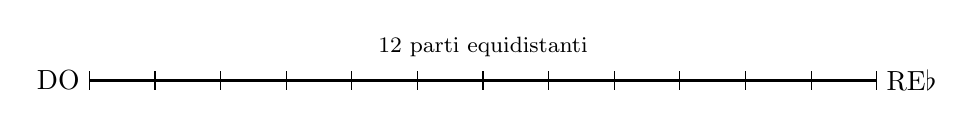
\begin{tikzpicture}[x=1cm,y=1cm]
    \draw[thick] (0,0) -- (10,0);
    \foreach \i in {0,...,12}{\draw (\i*10/12,-0.12) -- (\i*10/12,0.12);}
    \node[left] at (0,0) {DO};
    \node[right] at (10,0) {RE$\flat$};
    \node[above,font=\footnotesize] at (5,0.18) {12 parti equidistanti};
  \end{tikzpicture}
\end{figure}

\[
  \text{DO--RE}\flat = 1{,}059463094 \times 2 = 2{,}118926189
\]
(spazio di una nona minore); quindi si procede a ricavare il coefficiente:
\[
  \sqrt[12]{2{,}118926189} = 1{,}064575137\ldots
\]
Il coefficiente così ottenuto, moltiplicato 12 volte a partire da una frequenza
di $100$~Hz, darà una serie di altezze così composta:

\begin{center}\small
\begin{tabular}{r l@{\qquad\qquad}r l}
 1) & 100~Hz & 8)  & 154{,}9 \\
 2) & 106{,}4 & 9)  & 164{,}9 \\
 3) & 113{,}3 & 10) & 175{,}6 \\
 4) & 120{,}6 & 11) & 186{,}9 \\
 5) & 128{,}4 & 12) & 199     \\
 6) & 136{,}7 & 13) & 211{,}9 \\
 7) & 145{,}5 &     &         \\
\end{tabular}
\end{center}

Un'ulteriore possibilità è data dal dividere l'intervallo di ottava, o
qualsiasi altro intervallo, in modo multiplo, vale a dire prima diviso in un
numero arbitrario di parti e poi ciascuna di queste divisa ancora in un numero
arbitrario di sottoparti. Nell'esempio seguente l'ottava viene divisa in tre
parti, ognuna formata da una terza maggiore, e poi ogni terza maggiore viene a
sua volta suddivisa successivamente in 5, 6 e 7 sottoparti equidistanti.

\begin{figure}[htbp]
  \centering
  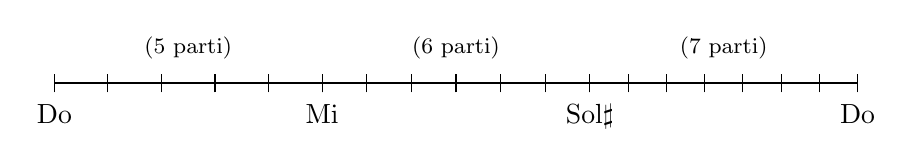
\begin{tikzpicture}[x=0.85cm,y=1cm]
    \draw[thick] (0,0) -- (12,0);
    % suddivisioni: Do-Mi 5 parti, Mi-Sol# 6 parti, Sol#-Do 7 parti
    \foreach \k in {0,...,5}{\draw (\k*4/5,-0.12) -- (\k*4/5,0.12);}
    \foreach \k in {0,...,6}{\draw (4+\k*4/6,-0.12) -- (4+\k*4/6,0.12);}
    \foreach \k in {0,...,7}{\draw (8+\k*4/7,-0.12) -- (8+\k*4/7,0.12);}
    \node[below] at (0,-0.15)  {Do};
    \node[below] at (4,-0.15)  {Mi};
    \node[below] at (8,-0.15)  {Sol$\sharp$};
    \node[below] at (12,-0.15) {Do};
    \node[above,font=\footnotesize] at (2,0.18)  {(5 parti)};
    \node[above,font=\footnotesize] at (6,0.18)  {(6 parti)};
    \node[above,font=\footnotesize] at (10,0.18) {(7 parti)};
  \end{tikzpicture}
\end{figure}

Essendo in questo caso l'ottava divisa in tre intervalli uguali (terze
maggiori), basterà trovare lo spazio di una sola terza maggiore:
\[
  \sqrt[12]{2} = 1{,}059463094^{4} = 1{,}25992105
\]
per poi procedere a trovare i tre diversi coefficienti:
\begin{align*}
  \text{Primo coefficiente}   &\quad \sqrt[5]{1{,}25992105} = 1{,}047294123 \\
  \text{Secondo coefficiente} &\quad \sqrt[6]{1{,}25992105} = 1{,}039259226 \\
  \text{Terzo coefficiente}   &\quad \sqrt[7]{1{,}25992105} = 1{,}033557783
\end{align*}
Ora, moltiplicando ciascun coefficiente per il numero delle rispettive
sottoparti nello spazio delle tre terze maggiori successive, partendo da una
frequenza di $100$~Hz, si otterrà un sistema di altezze così articolato:

\begin{center}\small
\begin{tabular}{r l@{\quad}r l@{\quad}r l}
1) & 100~Hz & 1) & 125{,}9 & 1) & 158{,}7 \\
2) & 104{,}7 & 2) & 130{,}9 & 2) & 164     \\
3) & 109{,}6 & 3) & 136     & 3) & 169{,}5 \\
4) & 114{,}8 & 4) & 141{,}4 & 4) & 175{,}2 \\
5) & 120{,}3 & 5) & 146{,}9 & 5) & 181{,}1 \\
6) & 125{,}9 & 6) & 152{,}7 & 6) & 187{,}3 \\
   &         & 7) & 158{,}7 & 7) & 193{,}5 \\
   &         &    &         & 8) & 200     \\
\end{tabular}
\end{center}

In generale, indicando con $n$, $m$ ed $l$ il numero delle sottoparti, le
altezze del sistema si ottengono con:
\[
  \sqrt[n]{\left(\sqrt[12]{2}\right)^{4}} \times
  \sqrt[m]{\left(\sqrt[12]{2}\right)^{4}} \times
  \sqrt[l]{\left(\sqrt[12]{2}\right)^{4}} \times f = \text{altezze}
\]

% =====================================================================
\section{Sistema di intonazione participato mesotonico}

Il sistema participato mesotonico è anche conosciuto come \emph{vecchio
temperamento ineguale} o \emph{nuovo temperamento}. Questo sistema, utilizzato
per oltre due secoli, riveste un ruolo preminente nella storia della musica
strumentale ed è stato per lungo tempo l'unico antagonista del temperamento
equabile. Difatti esso era in uso quasi universalmente nella pratica musicale
occidentale intorno al 1700. Fatto risalire a Gioseffo Zarlino
(\emph{Dimostrazioni harmoniche}, Venezia 1571) e allo spagnolo Francisco
Salinas (\emph{De Musica Libri VII}, Salamanca 1577), sebbene già ampiamente
spiegato nel trattato di Pietro Aron (\emph{Toscanello in musica}, Venezia
1523), pare avesse origini assai più remote (Bartolomeo Ramis e oltre). Questo
sistema, composto da terze maggiori naturali e quinte temperate, consiste nel
far combinare la terza maggiore risultante dalla serie di quattro quinte
consecutive (DO SOL RE LA MI) con la terza maggiore naturale risultante da due
ottave più una terza maggiore. Essendo l'intervallo risultante dalle quattro
quinte ($3 \times 3 \times 3 \times 3 = 81$) $81/64 = 81:64 = 404{,}8$ cents più
alto di un comma sintonico rispetto alla terza maggiore naturale
($5/4 = 386{,}3$ cents):
\[
  \frac{81}{64} \times \frac{4}{5} = \frac{324}{320} = \frac{81}{80}
\]
nel sistema participato ad un quarto di comma si è proceduto all'abbassamento
(temperamento o participazione) di ognuna delle quattro quinte successive di
$1/4$ di comma, $\sqrt[4]{5} = 1{,}49534 = 696{,}6$ cents invece di $1{,}5 = 702$
cents che caratterizza la quinta esatta, in modo tale che la quarta quinta
potesse essere di un intero comma sintonico più bassa e quindi coincidere con la
terza maggiore naturale.

Il nome di questo sistema deriva dal fatto che, in base a tale temperamento,
l'intervallo di un tono corrisponde alla media aritmetica tra il tono grande
$9/8$ e il tono piccolo $10/9$ del sistema naturale, in modo da ottenere che
l'intervallo di terza maggiore sia diviso in due toni di $193{,}2$ cents e
quindi esattamente uguali:
\[
  \frac{10}{9} \times \frac{9}{8} = \frac{5}{4} = 386{,}3~\text{cents}
\]
che diviso 2 darà appunto $193{,}2$ cents. Oppure, rispetto al sistema
pitagorico, il valore del tono medio sarà ricavato sommando i due toni $9/8$
abbassati ciascuno di mezzo comma sintonico e dividendo successivamente per 2:
\[
  \frac{9}{8} \times \frac{9}{8} = \frac{81}{64}
  \qquad
  \frac{81}{64} \times \frac{80}{81} = \frac{5}{4}
\]
La distinzione tra tono grande ($204$ cents) e tono piccolo ($182$ cents) viene
abolita dal tono medio ($193{,}2$ cents). Il semitono diatonico ($112$ cents)
diviene di $117{,}1$ cents e il semitono cromatico ($92$ cents) è di $76$ cents.

\begin{figure}[htbp]
  \centering\setlength{\tabcolsep}{4pt}
  \resizebox{\textwidth}{!}{%
  \begin{tabular}{*{13}{c}}
    Do & Do$\sharp$ & Re & Mi$\flat$ & Mi & Fa & Fa$\sharp$ & Sol & Sol$\sharp$
       & La & Si$\flat$ & Si & Do \\
    \addlinespace
    0 & 76 & 193,2 & 310,3 & 386,3 & 503,4 & 579,5 & 696,6 & 772,6 & 889,7
      & 1006,8 & 1082,9 & 1200 \\
  \end{tabular}}
\end{figure}

Questa procedura porta ad una scala che, rispetto a quella pitagorica, sarà così
configurata (v.\ schema del sistema mesotonico participato di $1/4$ di comma):

\begin{figure}[htbp]
  \centering
  \resizebox{\textwidth}{!}{%
  \begin{tabular}{l*{8}{c}}
    pitagorica: & Do & Re & Mi & Fa & Sol & La & Si & Do \\
                & 0 & 204 & 386,3 & 498 & 702 & 884 & 1088 & 1200 \\
    \addlinespace
    mesotonica: & Do & Re$^{-1/2}$ & Mi$^{-1}$ & Fa$^{+1/4}$ & Sol$^{-1/4}$
                & La$^{-3/4}$ & Si$^{-5/4}$ & Do \\
                & 0 & 193,2 & 386,2 & 503,4 & 696,6 & 889,7 & 1082,9 & 1200 \\
  \end{tabular}}
\end{figure}

e nella sua forma completa risulterà:

\begin{figure}[htbp]
  \centering\setlength{\tabcolsep}{5pt}
  \resizebox{\textwidth}{!}{%
  \begin{tabular}{*{13}{c}}
    Do & Do$\sharp^{-7/4}$ & Re$^{-1/2}$ & Mi$\flat^{+3/4}$ & Mi$^{-1}$
       & Fa$^{+1/4}$ & Fa$\sharp^{-3/2}$ & Sol$^{-1/4}$ & Sol$\sharp^{-2}$
       & La$^{-3/4}$ & Si$\flat^{+1/2}$ & Si$^{-5/4}$ & Do \\
  \end{tabular}}
\end{figure}

Da quanto detto precedentemente, l'intero sistema sarà pertanto ricavato da tre
serie di quattro quinte abbassate ciascuna di $1/4$ di comma sintonico (come
semplificazione rispetto a DO, due serie verso l'alto ed una verso il basso):

\begin{figure}[htbp]
  \centering
  \resizebox{\textwidth}{!}{%
  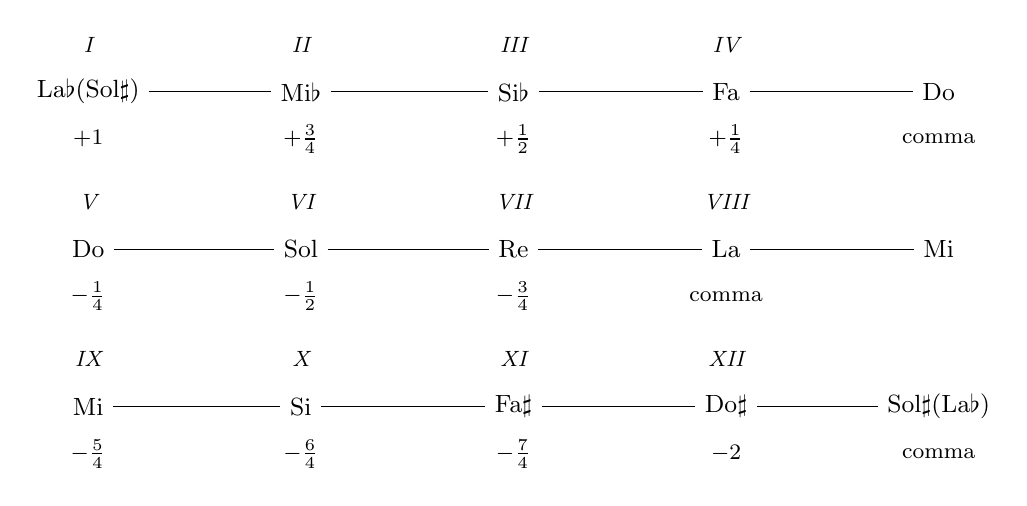
\begin{tikzpicture}[x=2.7cm,y=1cm,
      nota/.style={font=\small},
      rn/.style={font=\footnotesize\itshape},
      adj/.style={font=\footnotesize}]
    % --- serie A: verso il basso (bemolli) ---
    \foreach \x/\n/\r/\a in {%
        0/{La$\flat$(Sol$\sharp$)}/I/$+1$, 1/{Mi$\flat$}/II/$+\frac34$,
        2/{Si$\flat$}/III/$+\frac12$, 3/{Fa}/IV/$+\frac14$, 4/{Do}//comma}{
      \node[nota] (A\x) at (\x,4) {\n};
      \ifx\r\empty\else\node[rn] at (\x,4.6) {\r};\fi
      \node[adj] at (\x,3.4) {\a};
    }
    \draw (A0)--(A1)--(A2)--(A3)--(A4);
    % --- serie B: verso l'alto ---
    \foreach \x/\n/\r/\a in {%
        0/{Do}/V/$-\frac14$, 1/{Sol}/VI/$-\frac12$, 2/{Re}/VII/$-\frac34$,
        3/{La}/VIII/comma, 4/{Mi}//{}}{
      \node[nota] (B\x) at (\x,2) {\n};
      \ifx\r\empty\else\node[rn] at (\x,2.6) {\r};\fi
      \node[adj] at (\x,1.4) {\a};
    }
    \draw (B0)--(B1)--(B2)--(B3)--(B4);
    % --- serie C: verso l'alto (diesis) ---
    \foreach \x/\n/\r/\a in {%
        0/{Mi}/IX/$-\frac54$, 1/{Si}/X/$-\frac64$, 2/{Fa$\sharp$}/XI/$-\frac74$,
        3/{Do$\sharp$}/XII/$-2$, 4/{Sol$\sharp$(La$\flat$)}//comma}{
      \node[nota] (C\x) at (\x,0) {\n};
      \ifx\r\empty\else\node[rn] at (\x,0.6) {\r};\fi
      \node[adj] at (\x,-0.6) {\a};
    }
    \draw (C0)--(C1)--(C2)--(C3)--(C4);
  \end{tikzpicture}}
\end{figure}

Come risulta dallo schema, il LA$\flat$ temperato (prima nota della serie), per
effetto della somma dei $4/4$ di comma, è più alto di un intero comma sintonico
o $21{,}5$ cents rispetto al LA$\flat$ pitagorico, mentre il SOL$\sharp$ (ultima
nota della serie), per lo stesso motivo, è invece più basso di due commi o $43$
cents rispetto al SOL$\sharp$ pitagorico.

Sappiamo inoltre che, a causa del comma ditonico $531441/524288$ (vedi sistema
di intonazione pitagorico), il SOL$\sharp$ pitagorico è più alto del LA$\flat$
pitagorico (della stessa serie delle quinte pitagoriche, $12^{\text{a}}$ quinta)
di $23{,}5$ cents. Considerando quanto detto, il SOL$\sharp$ temperato finale
risulterà a questo punto $43 + 21{,}5 = 23{,}5 = 41$ cents più alto del
LA$\flat$ iniziale, temperato di circa $1/4$ di tono (differenza chiamata
\emph{Diesis}). Quindi l'intervallo di quinta SOL$\sharp$--Mi$\flat$ sarà
formato da $696{,}6$ (valore in cents della quinta temperata) $+ 41$ cents di
scarto $= 737{,}6$ cents. Questo intervallo di quinta, data la sua discordanza
rispetto alle altre, era chiamato \emph{quinte-de-loup} o \emph{quinta del
lupo}. Oltre a questa quinta si ha la presenza delle false terze Si--Mi$\flat$,
Fa$\sharp$--Si$\flat$, Do$\sharp$--Fa$\sharp$, Sol$\sharp$--Do.

Deve essere considerato anche che nella scala di Mi Maggiore dobbiamo impiegare
Mi$\flat$ al posto di Re$\sharp$ e questo conduce ancora ad un errore di $41$
cents, come pure avviene in quella di Mi$\flat$ che comporta l'introduzione di
Sol$\sharp$ al posto di La$\flat$. Tuttavia, per quanto il sistema mesotonico
risultasse soddisfacente sia melodicamente che armonicamente, a causa di tali
intervalli poteva essere impiegato soltanto in un ambito ristretto di tonalità
(da tre diesis a due bemolli). Un inconveniente del genere si poteva in parte
ovviare aumentando il numero degli intervalli nell'ottava. Vale la pena
ricordare a questo proposito come Nicola Vicentino, nel suo archicembalo a sei
tastiere, impiegava il sistema participato ordinario ottenendo così la divisione
dell'ottava in 31 parti ineguali.\footnote{Nicola Vicentino, \emph{L'antica
musica ridotta alla moderna prattica}, Roma 1555.}

Esistevano altre varietà di sistemi participati, oltre quello detto ordinario,
in cui le quinte venivano abbassate di $1/3$ o $1/5$ o $2/7$ di comma e persino
con varie combinazioni tra loro, ma il temperamento di $1/4$ di comma per quinta
risultò essere, nel suo complesso, il più soddisfacente
musicalmente.\footnote{R.~M.~H. Bosanquet, \emph{An Elementary Treatise on
Musical Intervals and Temperaments}, London 1876.}

\section{Costruzione di un sistema di intonazione non temperato}
% TODO trascrivere

\section{Sistema pitagorico}
% TODO trascrivere

\section{Tetracordo, generi e sistemi nella musica greca}
% TODO trascrivere

\subsection{Generi}
% TODO trascrivere

\subsection{Sistema perfetto}
% TODO trascrivere

\subsection{Nome delle corde della \emph{Lira} rispetto alle note nel
            collegamento di due tetracordi}
% TODO trascrivere

\subsection{Specie di ottava}
% TODO trascrivere

\section{Sistema naturale}
% TODO trascrivere

\section{Oltre il fattore 5}
% TODO trascrivere

\section{Altra possibilità di organizzazione degli intervalli derivante dai
         fattori generativi 2, 3 e 5}
% TODO trascrivere


% --------------------------- Appendici -------------------------------
% =====================================================================
%  Appendici 1-5  (scansione p-58 .. p-67)
%  STATO: tutte le appendici complete (1, 2, 3, 4, 5).
%  App. 3: 340 intervalli naturali nel rapporto 2/1; rapporti trascritti
%  dalle foto e verificati ricalcolando i cents (49/33 corretto da 49/35).
% =====================================================================
\newcommand{\appendice}[1]{%
  \chapter*{Appendice #1}%
  \addcontentsline{toc}{chapter}{Appendice #1}%
  \markboth{Appendice #1}{Appendice #1}%
}

% =====================================================================
\appendice{1}

\noindent Serie degli armonici fino al 16\textsuperscript{o} parziale, rapporti
assoluti e rapporti contenuti nello spazio di una sola ottava.

\begin{center}\small
\setlength{\tabcolsep}{8pt}
\renewcommand{\arraystretch}{1.15}
\resizebox{\textwidth}{!}{%
\begin{tabular}{cccc}
  \multicolumn{1}{c}{\textbf{I ottava}} & \multicolumn{1}{c}{\textbf{II ottava}}
  & \multicolumn{1}{c}{\textbf{III ottava}} & \multicolumn{1}{c}{\textbf{IV ottava}} \\[4pt]
        &        &        & $16 = \tfrac{16}{1} = \tfrac{1}{1}$ \\
        &        &        & $15 = \tfrac{15}{1} = \tfrac{15}{8}$ \\
        &        &        & $14 = \tfrac{14}{1} = \tfrac{7}{4}$ \\
        &        &        & $13 = \tfrac{13}{1} = \tfrac{13}{8}$ \\
        &        & $8 = \tfrac{8}{1} = \tfrac{1}{1}$ & $12 = \tfrac{12}{1} = \tfrac{3}{2}$ \\
        &        & $7 = \tfrac{7}{1} = \tfrac{7}{4}$ & $11 = \tfrac{11}{1} = \tfrac{11}{8}$ \\
        & $4 = \tfrac{4}{1} = \tfrac{1}{1}$ & $6 = \tfrac{6}{1} = \tfrac{3}{2}$ & $10 = \tfrac{10}{1} = \tfrac{5}{4}$ \\
  $2 = \tfrac{2}{1} = \tfrac{1}{1}$ & $3 = \tfrac{3}{1} = \tfrac{3}{2}$ & $5 = \tfrac{5}{1} = \tfrac{5}{4}$ & $9 = \tfrac{9}{1} = \tfrac{9}{8}$ \\
  $1 = \tfrac{1}{1}$ & $2 = \tfrac{2}{1} = \tfrac{1}{1}$ & $4 = \tfrac{4}{1} = \tfrac{1}{1}$ & $8 = \tfrac{8}{1} = \tfrac{1}{1}$ \\
\end{tabular}}
\end{center}

\bigskip
\noindent La stessa serie sviluppata a partire dal $1 = 261{,}6$~Hz (DO) e con
le rispettive note approssimate:

\begin{center}\small
\setlength{\tabcolsep}{8pt}
\renewcommand{\arraystretch}{1.15}
\resizebox{\textwidth}{!}{%
\begin{tabular}{cccc}
  \multicolumn{1}{c}{\textbf{I ottava}} & \multicolumn{1}{c}{\textbf{II ottava}}
  & \multicolumn{1}{c}{\textbf{III ottava}} & \multicolumn{1}{c}{\textbf{IV ottava}} \\[4pt]
        &        &        & $16 = 4185{,}6 = \text{DO}$ \\
        &        &        & $15 = 3924 = \text{SI}$ \\
        &        &        & $14 = 3662{,}4 = \text{SI}\flat$ \\
        &        &        & $13 = 3400{,}8 = \text{LA}$ \\
        &        & $8 = 2092{,}8 = \text{DO}$ & $12 = 3139{,}2 = \text{SOL}$ \\
        &        & $7 = 1831{,}2 = \text{SI}\flat$ & $11 = 2877{,}6 = \text{FA}\sharp$ \\
        & $4 = 1046{,}4 = \text{DO}$ & $6 = 1569{,}6 = \text{SOL}$ & $10 = 2616 = \text{MI}$ \\
  $2 = 523{,}2 = \text{DO}$ & $3 = 784{,}8 = \text{SOL}$ & $5 = 1308 = \text{MI}$ & $9 = 2354{,}4 = \text{RE}$ \\
  $1 = 261{,}6 = \text{DO}$ & $2 = 523{,}2 = \text{DO}$ & $4 = 1046{,}4 = \text{DO}$ & $8 = 2092{,}8 = \text{DO}$ \\
\end{tabular}}
\end{center}

% =====================================================================
\appendice{2}

\noindent Temperamento equabile dell'ottava divisa in 12 parti
($\sqrt[12]{2} = 1{,}0594631$) partendo da $\text{DO} = 261{,}6$~Hz; rispettive
frequenze e valori in cents.

\begin{center}
\renewcommand{\arraystretch}{1.1}
\begin{tabular}{lrr}
  \toprule
  \textbf{Nota} & \textbf{Frequenza} & \textbf{Cents} \\
  \midrule
  DO                       & 261,6 & 0 \\
  RE$\flat$ o DO$\sharp$   & 277,1 & 100 \\
  RE                       & 293,6 & 200 \\
  MI$\flat$ o RE$\sharp$   & 311,1 & 300 \\
  MI                       & 329,6 & 400 \\
  FA                       & 349,2 & 500 \\
  SOL$\flat$ o FA$\sharp$  & 369,9 & 600 \\
  SOL                      & 391,9 & 700 \\
  LA$\flat$ o SOL$\sharp$  & 415,3 & 800 \\
  LA                       & 440,0 & 900 \\
  SI$\flat$ o LA$\sharp$   & 466,1 & 1000 \\
  SI                       & 493,8 & 1100 \\
  DO                       & 523,2 & 1200 \\
  \bottomrule
\end{tabular}
\end{center}

% =====================================================================
\appendice{3}

% --- Appendice 3 (340 intervalli naturali) ---
\noindent 340 intervalli naturali nel rapporto $2/1$ e loro rispettivi valori
in cents.

\medskip
{\footnotesize
\setlength{\tabcolsep}{4pt}
\begin{longtable}{l r @{\qquad} l r @{\qquad} l r}
  \toprule
  intervallo & cents & intervallo & cents & intervallo & cents \\
  \midrule
  \endfirsthead
  \toprule
  intervallo & cents & intervallo & cents & intervallo & cents \\
  \midrule
  \endhead
  \midrule \endfoot
  \bottomrule \endlastfoot
$1/1$ & 0 & $32805/32768$ & 1{,}954 & $169/168$ & 10{,}3 \\
$144/143$ & 12{,}1 & $121/120$ & 14{,}4 & $105/104$ & 16{,}6 \\
$100/99$ & 17{,}4 & $99/98$ & 17{,}6 & $91/90$ & 19{,}1 \\
$81/80$ & 21{,}5 & $78/77$ & 22{,}3 & $531441/524288$ & 23{,}5 \\
$74/73$ & 23{,}6 & $66/65$ & 26{,}4 & $65/64$ & 26{,}8 \\
$64/63$ & 27{,}3 & $56/55$ & 31{,}2 & $55/54$ & 31{,}8 \\
$50/49$ & 35 & $49/48$ & 35{,}7 & $45/44$ & 38{,}9 \\
$6561/6400$ & 43 & $40/39$ & 43{,}8 & $36/35$ & 48{,}8 \\
$33/32$ & 53{,}3 & $512/495$ & 58{,}5 & $648/625$ & 62{,}6 \\
$28/27$ & 63 & $80/77$ & 66{,}2 & $126/121$ & 70{,}1 \\
$25/24$ & 70{,}7 & $2673/2560$ & 74{,}8 & $22/21$ & 80{,}5 \\
$21/20$ & 84{,}5 & $81/77$ & 87{,}7 & $256/243$ & 90{,}2 \\
$135/128$ & 92{,}2 & $128/121$ & 97{,}4 & $200/189$ & 97{,}9 \\
$18/17$ & 99 & $196/185$ & 100 & $89/84$ & 100{,}1 \\
$35/33$ & 101{,}9 & $297/280$ & 102 & $17/16$ & 105 \\
$1701/1600$ & 106 & $1089/1024$ & 106{,}5 & $16/15$ & 111{,}7 \\
$2187/2048$ & 113{,}7 & $77/72$ & 116{,}2 & $15/14$ & 119{,}4 \\
$189/176$ & 123{,}4 & $14/13$ & 128{,}3 & $320/297$ & 129{,}1 \\
$27/25$ & 133{,}2 & $121/112$ & 133{,}8 & $693/640$ & 137{,}7 \\
$13/12$ & 138{,}6 & $243/224$ & 140{,}9 & $88/81$ & 143{,}5 \\
$160/147$ & 146{,}7 & $49/45$ & 147{,}4 & $12/11$ & 150{,}6 \\
$35/32$ & 155{,}1 & $800/729$ & 160{,}9 & $11/10$ & 165 \\
$54/49$ & 168{,}2 & $441/400$ & 168{,}9 & $243/220$ & 172{,}1 \\
$567/512$ & 176{,}6 & $256/231$ & 177{,}9 & $65536/59049$ & 180{,}4 \\
$10/9$ & 182{,}4 & $49/44$ & 186{,}3 & $891/800$ & 186{,}5 \\
$28/25$ & 196{,}2 & $121/108$ & 196{,}8 & $55/49$ & 200 \\
$9/8$ & 203{,}9 & $640/567$ & 209{,}7 & $112/99$ & 213{,}6 \\
$363/320$ & 218{,}3 & $25/22$ & 221{,}3 & $256/225$ & 223{,}5 \\
$729/640$ & 225{,}4 & $8/7$ & 231{,}2 & $63/55$ & 235{,}1 \\
$55/48$ & 235{,}7 & $147/128$ & 239{,}6 & $1024/891$ & 240{,}9 \\
$280/243$ & 245{,}4 & $231/200$ & 249{,}5 & $140/121$ & 252{,}5 \\
$81/70$ & 252{,}7 & $297/256$ & 257{,}2 & $512/441$ & 258{,}4 \\
$64/55$ & 262{,}4 & $220/189$ & 262{,}9 & $7/6$ & 266{,}9 \\
$90/77$ & 270{,}1 & $2560/2187$ & 272{,}6 & $75/64$ & 274{,}6 \\
$88/75$ & 276{,}7 & $33/28$ & 284{,}4 & $189/160$ & 288{,}4 \\
$13/11$ & 289{,}2 & $32/27$ & 294{,}1 & $44/37$ & 300 \\
$144/121$ & 301{,}3 & $25/21$ & 301{,}8 & $105/88$ & 305{,}8 \\
$176/147$ & 311{,}7 & $6/5$ & 315{,}6 & $19683/16384$ & 317{,}6 \\
$77/64$ & 320{,}1 & $135/112$ & 323{,}4 & $880/729$ & 325{,}9 \\
$98/81$ & 329{,}8 & $121/100$ & 330 & $40/33$ & 333 \\
$243/200$ & 337{,}1 & $128/105$ & 342{,}9 & $11/9$ & 347{,}4 \\
$60/49$ & 350{,}6 & $49/40$ & 351{,}3 & $27/22$ & 354{,}5 \\
$315/256$ & 359 & $16/13$ & 359{,}5 & $448/363$ & 364{,}2 \\
$100/81$ & 364{,}8 & $121/98$ & 365 & $99/80$ & 368{,}9 \\
$56/45$ & 378{,}6 & $96/77$ & 381{,}8 & $8192/6561$ & 384{,}4 \\
$5/4$ & 386{,}3 & $1120/891$ & 396 & $44/35$ & 396{,}2 \\
$63/50$ & 400{,}1 & $121/96$ & 400{,}7 & $512/405$ & 405{,}9 \\
$81/64$ & 407{,}8 & $80/63$ & 413{,}6 & $14/11$ & 417{,}5 \\
$32/25$ & 427{,}4 & $77/60$ & 431{,}9 & $9/7$ & 435{,}1 \\
$567/440$ & 439 & $165/128$ & 439{,}6 & $128/99$ & 444{,}8 \\
$35/27$ & 449{,}3 & $100/77$ & 452{,}5 & $13/10$ & 454{,}2 \\
$729/560$ & 456{,}6 & $176/135$ & 459{,}1 & $64/49$ & 462{,}3 \\
$72/55$ & 466{,}3 & $55/42$ & 466{,}9 & $21/16$ & 470{,}8 \\
$320/243$ & 476{,}5 & $33/25$ & 480{,}6 & $160/121$ & 483{,}7 \\
$297/224$ & 488{,}4 & $1701/1280$ & 492{,}3 & $4/3$ & 498 \\
$578/433$ & 500 & $147/110$ & 502 & $162/121$ & 505{,}2 \\
$75/56$ & 505{,}8 & $121/90$ & 512{,}4 & $400/297$ & 515{,}4 \\
$66/49$ & 515{,}6 & $27/20$ & 519{,}6 & $177147/131072$ & 521{,}5 \\
$693/512$ & 524{,}1 & $256/189$ & 525{,}3 & $224/165$ & 529{,}2 \\
$110/81$ & 529{,}8 & $200/147$ & 533 & $49/36$ & 533{,}7 \\
$15/11$ & 537 & $2187/1600$ & 541{,}1 & $48/35$ & 546{,}8 \\
$11/8$ & 551{,}3 & $441/320$ & 555{,}2 & $243/176$ & 558{,}5 \\
$112/81$ & 561 & $18/13$ & 563{,}4 & $320/231$ & 564{,}2 \\
$168/121$ & 568{,}1 & $25/18$ & 568{,}7 & $891/640$ & 572{,}8 \\
$88/63$ & 578{,}6 & $7/5$ & 582{,}5 & $108/77$ & 585{,}7 \\
$1024/729$ & 588{,}3 & $45/32$ & 590{,}2 & $512/363$ & 595{,}4 \\
$800/567$ & 596 & $140/99$ & 599{,}9 & $99/70$ & 600{,}1 \\
$567/400$ & 604 & $363/256$ & 604{,}6 & $64/45$ & 609{,}8 \\
$729/512$ & 611{,}7 & $77/54$ & 614{,}3 & $10/7$ & 617{,}5 \\
$63/44$ & 621{,}4 & $1280/891$ & 627{,}2 & $36/25$ & 631{,}3 \\
$121/84$ & 631{,}9 & $231/160$ & 635{,}8 & $13/9$ & 636{,}6 \\
$81/56$ & 639 & $352/243$ & 641{,}5 & $640/441$ & 644{,}8 \\
$16/11$ & 648{,}7 & $35/24$ & 653{,}2 & $3200/2187$ & 658{,}9 \\
$22/15$ & 663 & $72/49$ & 666{,}3 & $147/100$ & 667 \\
$81/55$ & 670{,}2 & $165/112$ & 670{,}8 & $189/128$ & 674{,}7 \\
$1024/693$ & 675{,}9 & $262144/177147$ & 678{,}5 & $40/27$ & 680{,}4 \\
$49/33$ & 684{,}4 & $297/200$ & 684{,}6 & $180/121$ & 687{,}6 \\
$112/75$ & 694{,}2 & $121/81$ & 694{,}8 & $220/147$ & 698 \\
$433/289$ & 700 & $3/2$ & 701{,}955~(702) & $2560/1701$ & 707{,}7 \\
$448/297$ & 711{,}6 & $121/80$ & 716{,}3 & $50/33$ & 719{,}4 \\
$243/160$ & 723{,}5 & $32/21$ & 729{,}2 & $84/55$ & 733{,}1 \\
$55/36$ & 733{,}7 & $49/32$ & 737{,}7 & $135/88$ & 740{,}9 \\
$1120/729$ & 743{,}4 & $20/13$ & 745{,}8 & $77/50$ & 747{,}5 \\
$54/35$ & 750{,}7 & $99/64$ & 755{,}2 & $256/165$ & 760{,}4 \\
$880/567$ & 761 & $14/9$ & 764{,}9 & $120/77$ & 768{,}1 \\
$25/16$ & 772{,}6 & $11/7$ & 782{,}5 & $63/40$ & 786{,}4 \\
$128/81$ & 792{,}2 & $405/256$ & 794{,}1 & $192/121$ & 799{,}3 \\
$100/63$ & 799{,}9 & $35/22$ & 803{,}8 & $891/560$ & 804 \\
$8/5$ & 813{,}7 & $6561/4096$ & 815{,}6 & $77/48$ & 818{,}2 \\
$45/28$ & 821{,}4 & $160/99$ & 831{,}1 & $196/121$ & 835 \\
$81/50$ & 835{,}2 & $363/224$ & 835{,}8 & $13/8$ & 840{,}5 \\
$512/315$ & 841 & $44/27$ & 845{,}5 & $80/49$ & 848{,}7 \\
$49/30$ & 849{,}4 & $18/11$ & 852{,}6 & $105/64$ & 857{,}1 \\
$400/243$ & 862{,}9 & $33/20$ & 867 & $200/121$ & 870 \\
$81/49$ & 870{,}2 & $729/440$ & 874{,}1 & $224/135$ & 876{,}6 \\
$128/77$ & 879{,}9 & $32768/19683$ & 882{,}4 & $5/3$ & 884{,}4 \\
$147/88$ & 888{,}3 & $176/105$ & 894{,}2 & $42/25$ & 898{,}2 \\
$121/72$ & 898{,}7 & $37/22$ & 900 & $27/16$ & 905{,}9 \\
$22/13$ & 910{,}8 & $320/189$ & 911{,}6 & $56/33$ & 915{,}6 \\
$75/44$ & 923{,}3 & $128/75$ & 925{,}4 & $2187/1280$ & 927{,}4 \\
$77/45$ & 929{,}9 & $12/7$ & 933{,}1 & $189/110$ & 937{,}1 \\
$55/32$ & 937{,}6 & $441/256$ & 941{,}6 & $512/297$ & 942{,}8 \\
$140/81$ & 947{,}3 & $121/70$ & 947{,}5 & $400/231$ & 950{,}5 \\
$243/140$ & 954{,}6 & $891/512$ & 959{,}1 & $256/147$ & 960{,}4 \\
$96/55$ & 964{,}3 & $110/63$ & 964{,}9 & $7/4$ & 968{,}8 \\
$1280/729$ & 974{,}6 & $225/128$ & 976{,}5 & $44/25$ & 978{,}7 \\
$640/363$ & 981{,}7 & $99/56$ & 986{,}4 & $567/320$ & 990{,}3 \\
$16/9$ & 996{,}1 & $98/55$ & 1000 & $216/121$ & 1003{,}2 \\
$25/14$ & 1003{,}8 & $1600/891$ & 1013{,}5 & $88/49$ & 1013{,}7 \\
$9/5$ & 1017{,}6 & $59049/32768$ & 1019{,}6 & $231/128$ & 1022{,}1 \\
$1024/567$ & 1023{,}4 & $440/243$ & 1027{,}9 & $800/441$ & 1031{,}1 \\
$49/27$ & 1031{,}8 & $20/11$ & 1035 & $729/400$ & 1039{,}1 \\
$64/35$ & 1044{,}9 & $11/6$ & 1049{,}4 & $90/49$ & 1052{,}6 \\
$147/80$ & 1053{,}3 & $81/44$ & 1056{,}5 & $448/243$ & 1059{,}1 \\
$24/13$ & 1061{,}4 & $1280/693$ & 1062{,}3 & $224/121$ & 1066{,}2 \\
$50/27$ & 1066{,}8 & $297/160$ & 1070{,}9 & $13/7$ & 1071{,}7 \\
$352/189$ & 1076{,}6 & $28/15$ & 1080{,}6 & $144/77$ & 1083{,}8 \\
$4096/2187$ & 1086{,}3 & $15/8$ & 1088{,}3 & $2048/1089$ & 1093{,}5 \\
$3200/1701$ & 1094 & $32/17$ & 1095 & $560/297$ & 1098 \\
$66/35$ & 1098{,}1 & $168/89$ & 1099{,}9 & $185/98$ & 1100 \\
$17/9$ & 1101 & $189/100$ & 1102{,}1 & $121/64$ & 1102{,}6 \\
$256/135$ & 1107{,}8 & $243/128$ & 1109{,}8 & $154/81$ & 1112{,}3 \\
$40/21$ & 1115{,}5 & $21/11$ & 1119{,}5 & $5120/2673$ & 1125{,}2 \\
$48/25$ & 1129{,}3 & $121/63$ & 1129{,}9 & $77/40$ & 1133{,}8 \\
$27/14$ & 1137 & $625/324$ & 1137{,}4 & $495/256$ & 1141{,}5 \\
$64/33$ & 1146{,}7 & $35/18$ & 1151{,}2 & $39/20$ & 1156{,}2 \\
$12800/6561$ & 1157 & $88/45$ & 1161{,}1 & $96/49$ & 1164{,}3 \\
$49/25$ & 1165 & $108/55$ & 1168{,}2 & $55/28$ & 1168{,}8 \\
$63/32$ & 1172{,}7 & $128/65$ & 1173{,}2 & $65/33$ & 1173{,}6 \\
$73/37$ & 1176{,}4 & $1048576/531441$ & 1176{,}5 & $77/39$ & 1177{,}7 \\
$160/81$ & 1178{,}5 & $180/91$ & 1180{,}9 & $196/99$ & 1182{,}4 \\
$99/50$ & 1182{,}6 & $208/105$ & 1183{,}4 & $240/121$ & 1185{,}6 \\
$143/72$ & 1187{,}9 & $336/169$ & 1189{,}7 & $65536/32805$ & 1198{,}046 \\
$2/1$ & 1200 &  &  &  &  \\
\end{longtable}
}

% =====================================================================
\appendice{4}

\begin{center}
\textbf{Potenze di 2}\\[6pt]
\small
\renewcommand{\arraystretch}{1.05}
\begin{tabular}{rr@{\qquad\qquad}rr}
\toprule
\multicolumn{2}{c}{} & \multicolumn{2}{c}{} \\[-12pt]
$2^{2}$ & 4 & $2^{23}$ & 8388608 \\
$2^{3}$ & 8 & $2^{24}$ & 16777216 \\
$2^{4}$ & 16 & $2^{25}$ & 33554432 \\
$2^{5}$ & 32 & $2^{26}$ & 67108864 \\
$2^{6}$ & 64 & $2^{27}$ & 134217728 \\
$2^{7}$ & 128 & $2^{28}$ & 268435456 \\
$2^{8}$ & 256 & $2^{29}$ & 536870912 \\
$2^{9}$ & 512 & $2^{30}$ & 1073741824 \\
$2^{10}$ & 1024 & $2^{31}$ & 2147483648 \\
$2^{11}$ & 2048 & $2^{32}$ & 4294967296 \\
$2^{12}$ & 4096 & $2^{33}$ & 8589934592 \\
$2^{13}$ & 8192 & $2^{34}$ & 17179869184 \\
$2^{14}$ & 16384 & $2^{35}$ & 34359738368 \\
$2^{15}$ & 32768 & $2^{36}$ & 68719476736 \\
$2^{16}$ & 65536 & $2^{37}$ & 137438953472 \\
$2^{17}$ & 131072 & $2^{38}$ & 274877906944 \\
$2^{18}$ & 262144 & $2^{39}$ & 549755813888 \\
$2^{19}$ & 524288 & $2^{40}$ & 1099511627776 \\
$2^{20}$ & 1048576 & $2^{41}$ & 2199023255552 \\
$2^{21}$ & 2097152 & $2^{42}$ & 4398046511104 \\
$2^{22}$ & 4194304 & $2^{43}$ & 8796093022208 \\
\bottomrule
\end{tabular}
\end{center}

\bigskip
\begin{center}
\textbf{Potenze di 3}\\[6pt]
\small
\renewcommand{\arraystretch}{1.05}
\begin{tabular}{rr@{\qquad\qquad}rr}
\toprule
\multicolumn{2}{c}{} & \multicolumn{2}{c}{} \\[-12pt]
$3^{2}$ & 9 & $3^{15}$ & 14348907 \\
$3^{3}$ & 27 & $3^{16}$ & 43046721 \\
$3^{4}$ & 81 & $3^{17}$ & 129140163 \\
$3^{5}$ & 243 & $3^{18}$ & 387420489 \\
$3^{6}$ & 729 & $3^{19}$ & 1162261467 \\
$3^{7}$ & 2187 & $3^{20}$ & 3486784401 \\
$3^{8}$ & 6561 & $3^{21}$ & 10460353203 \\
$3^{9}$ & 19683 & $3^{22}$ & 31381059609 \\
$3^{10}$ & 59049 & $3^{23}$ & 94143178827 \\
$3^{11}$ & 177147 & $3^{24}$ & 282429536481 \\
$3^{12}$ & 531441 & $3^{25}$ & 847288609443 \\
$3^{13}$ & 1594323 & $3^{26}$ & 2541865828329 \\
$3^{14}$ & 4782969 & $3^{27}$ & 7625597484987 \\
\bottomrule
\end{tabular}
\end{center}

% =====================================================================
\appendice{5}

\begin{center}
\textbf{Numeri primi inferiori a 3000}\\[6pt]
\scriptsize
\setlength{\tabcolsep}{4pt}
\renewcommand{\arraystretch}{1.0}
\begin{tabular}{*{10}{r}}
\toprule
2 & 193 & 449 & 733 & 1031 & 1321 & 1637 & 1997 & 2333 & 2677 \\
3 & 197 & 457 & 739 & 1033 & 1327 & 1657 & 1999 & 2339 & 2683 \\
5 & 199 & 461 & 743 & 1039 & 1361 & 1663 & 2003 & 2341 & 2687 \\
7 & 211 & 463 & 751 & 1049 & 1367 & 1667 & 2011 & 2347 & 2689 \\
11 & 223 & 467 & 757 & 1051 & 1373 & 1669 & 2017 & 2351 & 2693 \\
13 & 227 & 479 & 761 & 1061 & 1381 & 1693 & 2027 & 2357 & 2699 \\
17 & 229 & 487 & 769 & 1063 & 1399 & 1697 & 2029 & 2371 & 2707 \\
19 & 233 & 491 & 773 & 1069 & 1409 & 1699 & 2039 & 2377 & 2711 \\
23 & 239 & 499 & 787 & 1087 & 1423 & 1709 & 2053 & 2381 & 2713 \\
29 & 241 & 503 & 797 & 1091 & 1427 & 1721 & 2063 & 2383 & 2719 \\
31 & 251 & 509 & 809 & 1093 & 1429 & 1723 & 2069 & 2389 & 2729 \\
37 & 257 & 521 & 811 & 1097 & 1433 & 1733 & 2081 & 2393 & 2731 \\
41 & 263 & 523 & 821 & 1103 & 1439 & 1741 & 2083 & 2399 & 2741 \\
43 & 269 & 541 & 823 & 1109 & 1447 & 1747 & 2087 & 2411 & 2749 \\
47 & 271 & 547 & 827 & 1117 & 1451 & 1753 & 2089 & 2417 & 2753 \\
53 & 277 & 557 & 829 & 1123 & 1453 & 1759 & 2099 & 2423 & 2767 \\
59 & 281 & 563 & 839 & 1129 & 1459 & 1777 & 2111 & 2437 & 2777 \\
61 & 283 & 569 & 853 & 1151 & 1471 & 1783 & 2113 & 2441 & 2789 \\
67 & 293 & 571 & 857 & 1153 & 1481 & 1787 & 2129 & 2447 & 2791 \\
71 & 307 & 577 & 859 & 1163 & 1483 & 1789 & 2131 & 2459 & 2797 \\
73 & 311 & 587 & 863 & 1171 & 1487 & 1801 & 2137 & 2467 & 2801 \\
79 & 313 & 593 & 877 & 1181 & 1489 & 1811 & 2141 & 2473 & 2803 \\
83 & 317 & 599 & 881 & 1187 & 1493 & 1823 & 2143 & 2477 & 2819 \\
89 & 331 & 601 & 883 & 1193 & 1499 & 1831 & 2153 & 2503 & 2833 \\
97 & 337 & 607 & 887 & 1201 & 1511 & 1847 & 2161 & 2521 & 2837 \\
101 & 347 & 613 & 907 & 1213 & 1523 & 1861 & 2179 & 2531 & 2843 \\
103 & 349 & 617 & 911 & 1217 & 1531 & 1867 & 2203 & 2539 & 2851 \\
107 & 353 & 619 & 919 & 1223 & 1543 & 1871 & 2207 & 2543 & 2857 \\
109 & 359 & 631 & 929 & 1229 & 1549 & 1873 & 2213 & 2549 & 2861 \\
113 & 367 & 641 & 937 & 1231 & 1553 & 1877 & 2221 & 2551 & 2879 \\
127 & 373 & 643 & 941 & 1237 & 1559 & 1879 & 2237 & 2557 & 2887 \\
131 & 379 & 647 & 947 & 1249 & 1567 & 1889 & 2239 & 2579 & 2897 \\
137 & 383 & 653 & 953 & 1259 & 1571 & 1901 & 2243 & 2591 & 2903 \\
139 & 389 & 659 & 967 & 1277 & 1579 & 1907 & 2251 & 2593 & 2909 \\
149 & 397 & 661 & 971 & 1279 & 1583 & 1913 & 2267 & 2609 & 2917 \\
151 & 401 & 673 & 977 & 1283 & 1597 & 1931 & 2269 & 2617 & 2927 \\
157 & 409 & 677 & 983 & 1289 & 1601 & 1933 & 2273 & 2621 & 2939 \\
163 & 419 & 683 & 991 & 1291 & 1607 & 1949 & 2281 & 2633 & 2953 \\
167 & 421 & 691 & 997 & 1297 & 1609 & 1951 & 2287 & 2647 & 2957 \\
173 & 431 & 701 & 1009 & 1301 & 1613 & 1973 & 2293 & 2657 & 2963 \\
179 & 433 & 709 & 1013 & 1303 & 1619 & 1979 & 2297 & 2659 & 2969 \\
181 & 439 & 719 & 1019 & 1307 & 1621 & 1987 & 2309 & 2663 & 2971 \\
191 & 443 & 727 & 1021 & 1319 & 1627 & 1993 & 2311 & 2671 & 2999 \\
\bottomrule
\end{tabular}
\end{center}


% --------------------------- Glossario -------------------------------
% =====================================================================
%  Glossario  (scansione p-70 .. p-71)
%  STATO: completo (voci da "Cent" a "Varietà di temperamento mesotonico"
%  più la tabella delle proporzioni matematiche/intervalli greci).
% =====================================================================
\chapter*{Glossario}
\addcontentsline{toc}{chapter}{Glossario}
\markboth{Glossario}{Glossario}

\voce{Cent}{Unità di misura dell'intervallo. La centesima parte di un semitono
temperato, con rapporto $\sqrt[1200]{2}$.}

\voce{Circolo delle quinte}{L'arrangiamento di note in un sistema chiuso di
quinte, come Do, Sol, Re, La, Mi, ecc.}

\voce{Comma}{Errore di intonazione, come nell'intervallo Si$\sharp$--Do nel
sistema pitagorico. Vedi \emph{Comma ditonico} e \emph{Comma sintonico}.}

\voce{Comma ditonico}{Intervallo tra 12 quinte e 7 ottave. Il suo rapporto è
$531441/524288$ ed è considerato convenzionalmente di 23,5 cents.}

\voce{Comma pitagorico}{Vedi \emph{Comma ditonico}.}

\voce{Comma sintonico}{Intervallo tra una terza maggiore naturale ($\rapp{5}{4}$)
e la terza pitagorica ($\rapp{81}{64}$). Il suo rapporto è $81/80$ ed è
considerato convenzionalmente di 21,5 cents.}

\voce{Comma tolematico}{Vedi \emph{Comma sintonico}.}

\voce{Diesis}{L'intervallo (circa $1/5$ di tono) tra due note enarmonicamente
equivalenti, come La$\flat$ e Sol$\sharp$, nell'intonazione naturale o nel
temperamento mesotonico. Il suo rapporto è $128/125$ di circa 41 cents.}

\voce{Divisione aritmetica}{Divisione uguale della differenza tra due quantità
tale che il risultato formi una progressione aritmetica; ad es.: $9:8:7:6$.}

\voce{Divisione geometrica}{Divisione proporzionale di due quantità, tale che il
risultato formi una progressione geometrica; ad es.: $27:18:12:8$.}

\voce{Divisione multipla}{Divisione dell'ottava in più di 12 parti, uguali o
ineguali.}

\voce{Epimorio}{Propriamente \enquote{una parte aggiunta}. È il termine usato
dai Greci per definire intervalli superparticolari. Vedi \emph{Rapporto
superparticolare}.}

\voce{Intonazione naturale}{Sistema d'intonazione basato sull'ottava
($\rapp{2}{1}$), la quinta pura ($\rapp{3}{2}$) e la terza maggiore pura
($\rapp{5}{4}$).}

\voce{Intonazione pitagorica}{Sistema d'intonazione basato sull'ottava
($\rapp{2}{1}$) e la quinta pura ($\rapp{3}{2}$).}

\voce{Monocordo}{Corda tesa su una base di legno sulla quale sono indicate le
lunghezze della corda per alcuni sistemi d'intonazione; diagramma che illustra
tali lunghezze; indicazioni per costruire tale diagramma.}

\voce{Quinta del lupo}{La quinta dissonante, usualmente Sol\#--Mi$\flat$ (notata
come sesta diminuita), presente in qualsiasi temperamento ineguale (tale che
sia di 737 cents anziché 702 cents).}

\voce{Rapporto superparticolare}{Un rapporto in cui l'antecedente eccede il
conseguente di 1, ad es. $\rapp{5}{4}$. Vedi \emph{Sesqui}.}

\voce{Schisma}{Differenza tra il comma sintonico e il comma ditonico, con
rapporto $32805/32768$, approssimativamente 2 cents.}

\voce{Sesqui}{Prefisso usato per designare un rapporto superparticolare, ad es.
la sesquiterza ($\rapp{4}{3}$).}

\voce{Sistema chiuso}{Un temperamento regolare in cui la nota iniziale si
ripresenta nuovamente.}

\voce{Sistema di intonazione}{Un sistema in cui tutti gli intervalli possono
essere espressi da numeri razionali.}

\voce{Temperamento equabile}{Divisione dell'ottava in un numero uguale di
parti, specificatamente in 12 semitoni, ciascuno dei quali ha rapporto
$\sqrt[12]{2}$.}

\voce{Temperamento ineguale}{Qualsiasi temperamento diverso da quello equabile,
particolarmente quello mesotonico o altre sue varietà.}

\voce{Temperamento mesotonico}{Propriamente un sistema di intonazione con
quinte abbassate e terze maggiori pure ($\rapp{5}{4}$). Vedi anche
\emph{Varietà di temperamento mesotonico}.}

\voce{Temperamento regolare}{Temperamento in cui tutte le quinte eccetto una
sono delle medesime dimensioni, come ad es. il sistema pitagorico o il
temperamento mesotonico (il temperamento equabile, con tutte le quinte uguali,
è anch'esso un temperamento regolare, così pure i sistemi chiusi di divisione
multipla).}

\voce{Temperare}{Variare leggermente l'altezza; specificatamente di una quinta
temperata.}

\voce{Varietà di temperamento mesotonico}{Temperamenti regolari basati sullo
stesso principio del temperamento mesotonico, con quinte abbassate e terze
alterate.}

\bigskip
\begin{center}
\textbf{Proporzioni matematiche e rispettivi intervalli musicali}\\[4pt]
\begin{tabular}{@{}lll@{}}
\toprule
Rapporto & Nome latino & Intervallo greco \\
\midrule
$\rapp{2}{1}$ & Dupla            & Diapason \\
$\rapp{3}{1}$ & Tripla           & Diapason Diapente \\
$\rapp{4}{1}$ & Quadrupla        & Bis Diapason \\
$\rapp{3}{2}$ & Sesquialtera     & Diapente \\
$\rapp{4}{3}$ & Sesquiterza      & Diatessaron \\
$\rapp{5}{4}$ & Sesquiquarta     & Diatonus Semitonus \\
$\rapp{8}{3}$ & Dupla Superbipartiens & Diapason Diatessaron \\
$\rapp{9}{8}$ & Sesquiottava     & Tonus \\
\bottomrule
\end{tabular}
\end{center}


% =====================================================================
%  BIBLIOGRAFIA
% =====================================================================
\backmatter
\chapter*{Bibliografia}
\addcontentsline{toc}{chapter}{Bibliografia}
\markboth{Bibliografia}{Bibliografia}
\nocite{*}                       % elenco completo (non citazioni puntuali)
\printbibliography[heading=none]

\end{document}
